\documentclass[12pt]{article}

\usepackage{svg}
\svgpath{{img/}}

\usepackage[T2A]{fontenc}
\usepackage[utf8]{inputenc}
\usepackage[english,russian]{babel}

\usepackage{amsmath}
\usepackage{amsthm, mathrsfs, mathtools, amssymb}
\usepackage{enumitem}

\usepackage{physics}

\renewcommand{\qedsymbol}{$\blacksquare$}
\theoremstyle{plain}
\newtheorem{theorem}{Теорема}

\usepackage{epigraph}

\usepackage{tikz}
\usepackage{subcaption}
\usetikzlibrary{decorations.pathmorphing}
% для волнистой линии для фотонов создал стиль линии snake arrow
% рисует волну и на конце ее чуть-чуть прямую линию оставляет для стрелки
\tikzset{snake arrow/.style=
	{->,
		decorate,
		decoration={snake,amplitude=.4mm,segment length=2mm,post length=1mm}},
}
\usepackage{caption}
\usepackage{float}
\usepackage{multirow}
\usepackage{multicol}
\usepackage{wrapfig}
\usepackage{hyperref}
\hypersetup{
		colorlinks,
		citecolor=black,
		filecolor=black,
		linkcolor=black,
		urlcolor=black
	}

\usepackage{geometry}
\geometry{verbose,a4paper,tmargin=1cm,bmargin=2cm,lmargin=1.5cm,rmargin=1.5cm}

\begin{document}
	%  \tableofcontents \newpage
	
	\begin{center}
		\LARGE \bf	
		\textsc{Уравнения математической физики}
		\rule{\textwidth}{0.4pt}
	\end{center}
	
	\section{Теоретическая часть}
	
	\subsection{Линейные уравнения с частными производными первого порядка. Уравнения характеристик. Первый интеграл. Квазилинейные уравнения. Задача Коши.}
\label{firstorder_lineq}

%autor: Сеня

\textit{Линейным уравнением с частными производными первого порядка} называется уравнение 
\begin{equation*}
	a_1 \frac{\partial u}{\partial x_1} + \dotsc + a_n \frac{\partial u}{\partial x_n} = b, \quad a_k = a_k(x_1, \dotsc, x_n), b = b(x_1, \dotsc, x_n).
\end{equation*}

Уравнение $\dot{x} = a(x)$ называется уравнением характеристик.
\textit{Пример:} Для уравнения $\partial u / \partial x = y \partial u / \partial y$ уравнениями характеристик будут $\dot{x} = 1, \dot{y} = -y$. 

Функция $f$ называется \textit{первым интегралом} уравнения $\dot{x} = v(x)$, если ее производная по направлению поля $v$ равна нулю:
\begin{equation*}
	v_1 \frac{\partial f}{\partial x_1} + \dotsc + v_n \frac{\partial f}{\partial x_n} = 0.
\end{equation*}

Отсюда легко понять, что функция $u$ является решением однородного линейного уравнения с частными производными первого порядка, если и только если она является первым интегралом уравнения характеристик. 

\textit{Квазилинейным уравнением первого порядка называется} уравнение
\begin{equation*}
	a_1(\textbf{x}, u) \frac{\partial u}{\partial x_1} + \dotsc + a_n(\textbf{x}, u) \frac{\partial u}{\partial x_n} = b(\textbf{x}, u).
\end{equation*}

\textit{Задачей Коши} называется задача нахождения решений уравнения 
\begin{equation*}
	a_1(x_1, \dotsc, x_n, u) \frac{\partial u}{\partial x_1} + \dotsc + a_n(x_1, \dotsc, x_n, u) \frac{\partial u}{\partial x_n} = b(x_1, \dotsc, x_n, u) 
\end{equation*}
с заданной начальной функцией
\begin{equation*}
	u|_{
	\gamma} = \varphi
\end{equation*}
определяющей значения функции на поверхности $(n - 1)$-мерной.
 \newpage
	\subsection{Классификация линейных уравнений с частными производными 2-го порядка. Характеристическое уравнение. Приведение уравнения с частными производными к каноническому виду.}
\label{sec:types}

%TODO: Характеристическое уравнение
%autor: Сеня

\paragraph{Классификация уравнений второго порядка.}
Уравнением с частными производными 2-го порядка называется:\footnote{Т.-С. стр. 15 и далее}
\begin{equation}
	F(x, y, u, u_x, u_y, u_{xx}, u_{xy}, u_{yy}) = 0.
\end{equation}

Уравнение называется линейным относительно старших производных, если оно имеет вид
\begin{equation} \label{SOlineq}
	a_{11}(x, y) u_{xx} + 2 a_{12}(x, y) u_{xy} + a_{22}(x, y) y_{yy} + F_1(x, y, u, u_x, u_y) = 0.
\end{equation}
\textit{Линейное} уравнение линейно относительно всех вхождений $u$. 

Линейные уравнения с частными производными 2-го порядка называются \textit{квазилинейными}, если коэффициенты $a_{11}, a_{12}, a_{22}$ зависят от $x, y, u, u_x, u_y$. 

\paragraph{Приведение уравнения к каноническому виду.}
%TODO: Сократить
С помощью преобразования переменных
\begin{equation*}
	\xi = \varphi(x, y), \quad \eta = \psi(x, y),
\end{equation*}
допускающего обратное преобразование, мы получаем новое уравнение, эквивалентное исходному. Как выбрать $\xi$ и $\eta$ так, чтобы получить наиболее простой вид?

Получим ответ на поставленный вопрос для \eqref{SOlineq}. Преобразуя производные к новым переменным, получаем
\begin{equation} \label{varchange}
	\begin{rcases}
		u_x = u_{\xi} \xi_{x} + u_{\eta} \eta_{x}, \\
		u_y = u_{\xi} \xi_{y} + u_{\eta} \eta_{y}, \\
		u_{xx} = u_{\xi\xi} \xi_{x}^2 + 2 u_{\xi\eta} \xi_{x} \eta_{x} + u_{\eta\eta} \eta^2_{x} + u_{\xi} \xi_{xx} + u_{\eta} \eta_{xx}, \\
		u_{xy} = u_{\xi\xi} \xi_{x} \xi_{y} + u_{\xi\eta}(\xi_x \eta_y + \xi_y \eta_x) + u_{\eta\eta} \eta_x \eta_y + u_{\xi} \xi_{xy} + u_{\eta} \eta_{xy}, \\
		u_{yy} = u_{\xi\xi} \xi_{y}^2 + 2 u_{\xi\eta} \xi_{y} \eta_{y} + u_{\eta\eta} \eta^2_{y} + u_{\xi} \xi_{yy} + u_{\eta} \eta_{yy},
	\end{rcases}
\end{equation}
Подставляя значения производных из \eqref{varchange} в уравнение \eqref{SOlineq}, будем иметь 
\begin{equation} \label{SOeqCHANGED}
	\bar{a}_{11} u_{\xi\xi} + 2 \bar{a}_{12} u_{\xi\eta} + \bar{a}_{22} u_{\eta\eta} + \bar{F} = 0,
\end{equation}
где 
\begin{align*}
	&\bar{a}_{11} = a_{11} \xi^2_{x} + 2 a_{12} \xi_x \xi_y + a_{22} \xi^2_y, \\
	&\bar{a}_{12} = a_{11} \xi_x \eta_x + a_{12} (\xi_x \eta_y + \eta_x \xi_y) + a_{22} \xi_{y} \eta_{y}, \\
	&\bar{a}_{22} = a_{11} \eta^2_{x} + 2 a_{12} \eta_x \eta_y + a_{22} \eta^2_y,
\end{align*}
а функция $\bar{F}$ не зависит от вторых производных. Заметим, что если исходное уравнение линейно, т.е. 
\begin{equation*}
	F(x, y, u, u_x, u_y) = b_1 u_x + b_2 u_y + c u + f,
\end{equation*}
то $\bar{F}$ имеет вид 
\begin{equation*}
	\bar{F}(\xi, \eta, u, u_{\xi}, u_{\eta}) = \beta_1 u_{\xi} + \beta_2 u_{\eta} + \gamma u + \delta,
\end{equation*}
т.е. уравнение остается линейным. 

Выберем переменные $\xi$ и $\eta$ так, чтобы коэффициент $\bar{a}_{11}$ был равен нулю. Рассмотрим уравнение с частными производными 1-го порядка
\begin{equation} \label{FOeq}
	a_{11} z^2_x + 2 a_{12} z_x z_y + a_{22} z_y^2 = 0.
\end{equation}
Если положить что $\xi = \varphi(x, y) = z_{\text{частное}}$, то коэффициент $\bar{a}_{11}$, очевидно, будет равен нулю. Таким образом, упомянутая выше задача о выборе новых независимых переменных связана с решением уравнения \eqref{FOeq}.  

Соотношение $\varphi(x, y) = C$ представляет собой общий интеграл обыкновенного дифференциального уравнения 
\begin{equation} \label{chareq}
	a_{11} dy^2 - 2 a_{12} dx dy + a_{22} dx^2 = 0.
\end{equation}

Если $\varphi(x, y) = C$ представляет собой общий интеграл обыкновенного дифференциального уравнения \eqref{chareq}, то функция $z = \varphi(x, y)$ удовлетворяет уравнению \eqref{FOeq}. 

Уравнение \eqref{chareq} называется \textit{характеристическим} для уравнения \eqref{SOlineq}, а его интегралы - \textit{характеристиками}. 

Пологая $\xi = \varphi(x, y)$, где $\varphi(x, y) = const$ есть общий интеграл уравнения \eqref{chareq}, мы обращаем в нуль коэффициент при $u_{\xi\xi}$. Если $\psi(x, y) = const$ является другим общим интегралом уравнения \eqref{chareq}, независимым от $\varphi(x, y)$, то, пологая $\eta = \psi(x, y)$, мы обратим в нуль также и коэффициент при $u_{\eta\eta}$. 

Уравнение \eqref{chareq} распадается на два уравнения:
\begin{align}
	\frac{dy}{dx} = \frac{a_{12} + \sqrt{a_{12}^2 - a_{11} a_{22}}}{a_{11}}, \\
	\frac{dy}{dx} = \frac{a_{12} - \sqrt{a_{12}^2 - a_{11} a_{22}}}{a_{11}}.
\end{align}

Знак подкоренного выражения определяет тип уравнения \eqref{SOlineq}
\begin{equation*}
	a_{11} u_{xx} + 2 a_{12} u_{xy} + a_{22} u_{yy} + F = 0.
\end{equation*}

Это уравнение мы будем называть в точке $M$ уравнением:
\begin{align*}
	&\texttt{гиперболического } \text{типа, если в точке } M \, \, a_{12}^2 - a_{11} a_{22} > 0, \\
	&\texttt{параболического } \text{типа, если в точке } M \,\, a_{12}^2 - a_{11} a_{22} = 0, \\
	&\texttt{эллиптического } \text{типа, если в точке } M \,\, a_{12}^2 - a_{11} a_{22} < 0.
\end{align*}

Рассмотрим область $G$, во всех точках которой уравнение имеет один и тот же тип. Через каждую точку области $G$ проходят две характеристики, причем для уравнений гиперболического типа характеристики действительны и различны, для уравнений эллиптического типа - комплексны и различны, а для уравнений параболического типа обе характеристики действительны и совпадают между собой. 

Для каждого из типов можно вывести каноническую форму уравнения.
\begin{enumerate}
	\item Каноническая форма уравнений гиперболического типа ($a_{12}^2 - a_{11} a_{22} > 0$) \begin{equation}
		u_{xx} - u_{yy} = \Phi \text{ или } u_{xy} = \Phi.
	\end{equation}
	
	\item Для уравнений параболического типа ($a_{12}^2 - a_{11} a_{22} = 0$)
	\begin{equation}
		u_{xx} = \Phi.
	\end{equation}
	
	\item Для уравнений эллиптического типа ($a_{12}^2 - a_{11} a_{22} < 0$)
	\begin{equation}
		u_{xx} + u_{yy} = \Phi.
	\end{equation} 
	
	Во всех случаях $\Phi = -\frac{\bar{F}}{\bar{a}_{22}}$.
\end{enumerate}
 \newpage
	\subsection{Уравнение колебаний бесконечной струны (стержня). Задача Коши с начальными условиями. Формула Даламбера. Характеристики.}
\label{DalamberFormula}

%autor: Сеня


\paragraph{Решение уравнения колебаний бесконечной струны и получение формулы Даламбера.}
Имеем уравнение:
\begin{gather}
	u_{tt} - a^2 u_{xx} = 0, \label{kernel_prob} \\
	u |_{t = 0} = u_0(x), \quad u_t|_{t = 0} = u_1(x).
\end{gather}

Докажем лемму.

\textsc{Лемма.} Для того чтобы функция $u(x, t)$ была решением уравнения, необходимо и достаточно, чтобы она имела представление 
\begin{equation} \label{represofsol}
	u(x, t) = f(x - at) + g(x + at),
\end{equation}

\textsc{Доказательство.} Функция \eqref{represofsol} удовлетворяет уравнению \eqref{kernel_prob}, т.к. 
\begin{equation*}
	\frac{\partial^2 u}{\partial t^2} = a^2 f''(x - at) + a^2 g''(x + at) = a^2 \frac{\partial^2 u}{\partial x^2}.
\end{equation*}

Обратно, пусть функция $u(x, t)$ удовлетворяет уравнению \eqref{kernel_prob}, представим это уравнение в каноническом виде. Дифференциальные уравнения характеристик\footnote{Объясню в следующем параграфе} имеют вид 
\begin{gather*}
	\frac{u_{tt}}{u_{xx}} = a^2 \\
	\frac{d t^2}{d x^2} = a^2 \\
	\frac{dx}{dt} = - a, \quad \frac{dx}{dt} = a,
\end{gather*}
заменим переменные
\begin{equation*}
	\xi = x - a t, \quad \eta = x + a t
\end{equation*}
это приводит уравнение к каноническому виду
\begin{equation*}
	\frac{\partial^2 \tilde{u}}{\partial \xi \partial \eta} = 0.
\end{equation*}

Интегрируя это уравнение по $\xi$, получим
\begin{equation*}
	\frac{\partial \tilde{u}}{\partial \eta} = \chi(\eta),
\end{equation*}

Запишем функцию $\tilde{u}$, проинтегрировав по $\eta$:
\begin{equation*}
	\tilde{u}(\xi, \eta) = \int^{\eta} \chi(\eta') \, d\eta' + f(\xi) = f(\xi) + g(\eta).
\end{equation*}

Переходя к старым переменным $x$ и $t$ из последнего представления убеждаемся, что предположение верно. Лемма доказана.  


Вернемся к решению уравнения \eqref{kernel_prob}. Для того чтобы решение удовлетворяло начальным условиям, необхолимо, чтобы
\begin{equation*}
	f(x) + g(x) = u_0(x), \quad -a f'(x) + a g'(x) = u_1(x)
\end{equation*}
т.е. 
\begin{equation*}
	f(\xi) + g(\xi) = u_0(\xi), \quad g(\xi) - f(\xi) = \frac{1}{a} \int_{0}^{\xi} u_1(\xi') \, d\xi' + C,
\end{equation*}
решая относительно $f$ и $g$ найдем
\begin{align*}
	f(\xi) = \frac{1}{2} u_0(\xi) - \frac{1}{2 a} \int_{0}^{\xi} u_1(\xi') \, d\xi' - \frac{C}{2}, \\
	g(\eta) = \frac{1}{2} u_0(\eta) + \frac{1}{2 a} \int_{0}^{\eta} u_1(\xi') \, d\xi' + \frac{C}{2}.
\end{align*}

Подставляя полученные выражения в \eqref{represofsol}, получаем формулу Даламбера
\begin{equation*}
	u(x, t) = \frac{1}{2} [u_0(x + a t) + u_0(x - a t)] + \frac{1}{2 a} \int_{x - a t}^{x + a t} u_1(\xi) \, d\xi.
\end{equation*}

\paragraph{Про характеристики.}
 \newpage
	\subsection{Уравнение колебаний полубесконечной струны (стержня). Метод отражений.}

\begin{equation}
	\square_{a} = \frac{\partial^2}{\partial t^2} - a^2 \Delta
\end{equation}

Изложенный в пункте \ref{DalamberFormula} метод решения задачи Коши позволяет решать некоторые смешанные задачи для этого уравнения. Для определенности рассмотрим смешанную задачу, описыващую колебание полубесконечной струны $x > 0$ с закрепленным левым концом
\begin{equation} \label{x0cond}
	u |_{x = 0} = 0.
\end{equation}

Предварительно докажем, что всякое классическое решение $u(x, t)$ уравнения \eqref{infinite_string} в квадрате $x > 0$, $t > 0$, удовлетворяющее условию \eqref{x0cond} представляется в виде 
\begin{equation} \label{xg0condim}
	u(x, t) = g(x + a t) - g(-x + a t)
\end{equation}

Действительно, решение представляется в виде \eqref{general_int}, где $f(\xi) \in \mathcal{C}^2(\mathbb{R}^1)$ и $g(\eta) \in \mathcal{C}^2(\eta > 0)$. Отсюда, учитывая условие \eqref{x0cond}, получим
\begin{equation} 
	0 = f_1(-a t) + f_2(a t)
\end{equation}
отсюда и вытекает представление \eqref{xg0condim}. 

Построим решение смешанной задачи \eqref{infinite_string}, \eqref{inf_str_cond}, \eqref{x0cond}. Всякое классическое решение $u(x, t)$ этой задачи в силу \eqref{xg0condim} допускает нечетное продолжение $\tilde{u}(x, t)$ по $x$ класса $\mathcal{C}^2(\mathbb{R}^2)$, и это продолжение удовлетворяет уравнению \eqref{infinite_string} в $\mathbb{R}^2$.
\begin{figure}[H]
	\centering
	\begin{subfigure}{0.4\textwidth}
		\includegraphics[width=\textwidth]{img/mirror1.png}
		\caption{}
	\end{subfigure}
	\hspace{5mm}
	\begin{subfigure}{0.4\textwidth}
		\includegraphics[width=\textwidth]{img/mirror2.png}
		\caption{}
	\end{subfigure}
\end{figure}
Отсюда из условий \eqref{inf_str_cond} вытекает, что решение $\tilde{u}(x, t)$ удовлетворяет начальным условиям
\begin{equation}
	\tilde{u}|_{t = 0} = \tilde{u}_0(x), \quad \tilde{u}_t|_{t = 0} = \tilde{u}_1(x),
\end{equation}
где $\tilde{u}_0$ и $\tilde{u}_1$ --- нечетные продолжения функций $u_0$ и $u_1$ соответственно. Но решение такой задачи Коши единственно и представляется формулой Даламбера \eqref{dAlamber} с заменой $u_0$ на $\tilde{u}_0$ и $u_1$ на $\tilde{u}_1$, если $\tilde{u}_0 \in \mathcal{C}^2(\mathbb{R}^1)$ и $\tilde{u}_1 \in \mathcal{C}^1(\mathbb{R}^1)$. Последние условия будут выполнены, если
\begin{equation} \label{setcond}
	u_0 \in \mathcal{C}^2(x \geqslant 0), \quad u_1 \in \mathcal{C}^1(x \geqslant 0), \quad u_0(0) = u_0''(0) = u_1(0) = 0.
\end{equation}

Итак, если выполнены условия \eqref{setcond}, то решение задачи \eqref{infinite_string}, \eqref{inf_str_cond}, \eqref{x0cond} существует, единственно и задается формулой 
\begin{equation} \label{formula}
	u(x, t) = \frac{1}{2} [\tilde{u}_0(x + a t) + \tilde{u}_0(x - a t)] + \frac{1}{2 a} \int_{x - a t}^{x + a t} \tilde{u}_1(\xi) \, d\xi, \quad x \geqslant 0.
\end{equation}

Пусть $x - a t \geqslant 0$. Тогда
\begin{equation}
	\tilde{u}_0(x - a t) = \tilde{u}_0(x - a t), \quad \tilde{u}_1(\xi) = u_1(\xi), \quad \xi \geqslant x - a t \geqslant 0,
\end{equation}
и формула \eqref{formula} принимает вид 
\begin{equation}
	u(x, t) = \frac{1}{2} [u_0(x + a t) + u_0(x - a t)] + \frac{1}{2 a} \int_{x - a t}^{x + a t} u_1(\xi) \, d\xi, \quad x \geqslant at.
\end{equation}

Аналогичные рассуждения можно провести для $x - a t \leqslant 0$. 
%TODO: Провести и дописать \newpage
	\subsection{Энергия колебаний ограниченной струны. Теорема единственности для смешанной краевой задачи для уравнения колебаний струны.}

\paragraph{Энергия колебаний ограниченной струны.}

Найдем выражение для энергии поперечных колебаний струны $E = K + U$, где $K$ --- кинетическая и $U$ - потенциальная энергия. Элемент струны $dx$, движущийся со скоростью $v = u_t$, обладает кинетической энергией 
\begin{equation*}
	\frac{1}{2} m v^2 = \frac{1}{2} \rho(x) \, dx(u_t)^2 \quad (m = \rho \, dx)
\end{equation*}

Кинетическая энергия всей струны равна 
\begin{equation}
	K = \frac{1}{2} \int \limits_{0}^{l} \rho(x) [u_t(x, t)]^2 \, dx.
\end{equation}

Потенциальная энергия поперечных колебаний струны, имеющей при $t = t_0$ форму $u(x, t_0) = u_0(x)$, равна работе, которую надо совершить, чтобы струна перешла из положения равновесия в положение $u_0(x)$. Пусть функция $u(x, t)$ дает профиль струны в момент $t$, причем
\begin{equation*}
	u(x, 0) = 0, \quad u(x, t_0) = u_0(x).
\end{equation*}
Элемент $dx$ под действием равнодействующей сил натяжения 
\begin{equation*}
	T \frac{\partial u}{\partial x} \Big|_{x + dx} - T \frac{\partial u}{\partial x} \Big|_{x} = T u_{xx} \, dx
\end{equation*}
за время $dt$ проходит путь $u_t(x, t) \, dt$. Работа, производимая всей струной за время $dt$, равна
\begin{equation*}
	\Bigg\{\int \limits_{0}^{l} T_0 u_{xx} u_t \, dx \Bigg\} \, dt = \Bigg\{T_0 u_x u_t \Big|_{0}^{l} - \int \limits_{0}^{l} T_0 u_x u_{xt} \, dx \Bigg\} \, dt =  \Bigg\{-\frac{1}{2} \frac{d}{dt} \int \limits_{0}^{l} T_0 (u_x)^2 \, dx + T_0 u_x u_t \Big|_{0}^{l}\Bigg\} \, dt.
\end{equation*}
Интегрируя по $t$ от $0$ до $t_0$, получаем
\begin{equation*}
	-\frac{1}{2} \int \limits_{0}^{l} T_0(u_x)^2 \, dx \Big|_{0}^{t_0} + \int \limits_{0}^{t_0} T_)0 u_x u_t \Big|_{0}^{l} \, dt = -\frac{1}{2} \int \limits_{0}^{l} T_0 [u_x(x, t_0)]^2 \, dx + \int \limits_{0}^{t_0} T_0 u_x u_t \Big|_{0}^{l} \, dt.
\end{equation*}

Нетрудно выяснить смысл последнего слагаемого правой части этого равенства. Действительно, $T_0 u_x|_{x = 0}$ есть величина натяжения на конце струны $x = 0; \, u_t(0, t) \, dt$  --- перемещение этого конца, а интеграл 
\begin{equation}
	\int \limits_{0}^{t_0} T_0 u_x u_t|_{x = 0} \, dt
\end{equation}
представляет работу, которую надо затратить на перемещение конца $x = 0$. Аналогичный смысл имеет слагаемое, соответствующее $x = l$. 

Если концы струны закрепленны, то работа на них будет равна нулю (при этом $u(0, t) = 0, u_t(0, t) = 0$). Следовательно, при перемещении закрепленной на концах струны из положения равновесия $u = 0$ в положение $u_0(x)$ работа не зависит от способа перехода струны в это положение и равна 
\begin{equation}
	-\frac{1}{2} \int \limits_{0}^{l} T_0[u'_0(x)]^2 \, dx, 
\end{equation}
потенциальной энергии струны в момент $t = t_0$ с обратным знаком.

Таким образом, полная энергия струны равна
\begin{equation}
	E = \frac{1}{2} \int \limits_{0}^{l} [T_0(u_x)^2 + \rho(x)(u_t)^2] \, dx.
\end{equation}

Совершенно аналогично может быть получено выражение для потенциальной энергии продольных колебаний стержня. Впрочем, его можно получить также, исходя из формулы для потенциальной энергии упругого стержня
\begin{equation*}
	U = \frac{1}{2} k(\frac{l - l_0}{l_0})^2 l_0,
\end{equation*}
где $l_0$ --- начальная длина стержня, $l$ --- конечная длина. Отсюда непосредственно следует 
\begin{equation*}
	U = \frac{1}{2} \int \limits_{0}^{l} k(u_x)^2 \, dx.
\end{equation*}

\paragraph{Теорема единственности для смешанной краевой задачи для уравнения колебаний струны.}
 \newpage
	\subsection{Метод разделения переменных для уравнения колебаний на отрезке.}
%autor: Сеня

Метод разделения переменных, или метод Фурье является одним из наиболее распространенных методов решения уравнений с частными производными.\footnote{Т.-С. стр. 87 и далее}

Изложение этого метода проведем для задачи колебания струны, закрепленной на концах (т.е. на отрезке). 

Итак, будем искать решение уравнения 
\begin{equation} \label{oscil}
	u_{tt} = a^2 u_{xx},
\end{equation}
удовлетворяющее однородным граничным условиям 
\begin{equation} \label{bord_cond}
	u(0, t) = 0, u(l, t) = 0
\end{equation}
и начальным условиям 
\begin{equation} \label{init_cond}
	\begin{cases}
		u(x, 0) = \varphi(x),
		\\
		u_t(x, 0) = \psi(x).
	\end{cases}
\end{equation}

Уравнение \eqref{oscil} линейно и однородно, поэтому сумма частных решений также является решением этого уравнения. Имея достаточно большое число частных решений, можно попытаться при помощи суммирования их с некоторыми коэффициентами найти искомое решение. 

Поставим основную вспомогательную задачу.

\textit{Найти решение уравнения}
\begin{equation*}
	u_{tt} = a^2 u_{xx},
\end{equation*}
\textit{не равное тождественно нулю, удовлетворяющее однородным граничным условиям}
\begin{equation}
	\label{ucond}
	\begin{cases}
		u(0, t) = 0,
		\\
		u(l, t) = 0
	\end{cases}
\end{equation}
\textit{и представимое в виде произведения}
\begin{equation} \label{sol_form}
	u(x, t) = X(x) T(t),
\end{equation}
\textit{где $X(x)$ --- функция только переменного $x$, $T(t)$ --- функция только переменного $t$.}

Подставляя предполагаемую форму решения \eqref{sol_form} в уравнение \eqref{oscil}, получим 
\begin{equation*}
	X'' T = \frac{1}{a^2} T'' X,
\end{equation*}
или, после деления на $X T$,
\begin{equation} \label{need}
	\frac{X''(x)}{X(x)} = \frac{1}{a^2} \frac{T''(t)}{T(t)}.
\end{equation}

Чтобы функция \eqref{sol_form} была решением уравнения \eqref{oscil}, равенство \eqref{need} должно удовлетворяться тождественно, т.е. для всех значений назависимых переменных $0 < x < l$, $t > 0$. Правая часть равенства \eqref{need} является функцией только переменного $t$, а левая --- только $x$. Фиксируя, например, некоторое значение $x$ и меняя $t$ (или наоборот), получим, что правая и левая части равенства \eqref{need} при изменении своих аргементов сохраняют постоянное значение
\begin{equation} \label{comstlambd}
	\frac{X''(x)}{X(x)} = \frac{1}{a^2} \frac{T''(t)}{T(t)} = -\lambda,
\end{equation}
где $\lambda$ --- постоянная, которую для удобства последующих выкладок берем со знаком "минус", ничего не предполагая при этом о ее знаке.

Из соотношения \eqref{comstlambd} получаем обыкновенные дифференциальные уравнения для определения функций $X(x)$ и $T(t)$:
\begin{align}
	&X''(x) + \lambda X(x) = 0, \quad X(x) \not \equiv 0, \\
	&T''(t) + a^2 \lambda T(t) = 0, \quad T(t) \not \equiv 0. \label{Teq}
\end{align}

Граничные условия \eqref{bord_cond} дают
\begin{align*}
	u(0, t) = X(0) T(t) = 0, \\
	u(l, t) = X(l) T(t) = 0.
\end{align*}
Отсюда следует, что функция $X(x)$ должна удовлетворять дополнительным условиям 
\begin{equation}
	X(0) = X(l) = 0,
\end{equation}
так как иначе мы имели бы
\begin{equation*}
	T(t) \equiv 0 \text{ и } u(x, t) \equiv 0,
\end{equation*}
в то время как задача состоит в нахождении нетривиального решения. Для функции $T(t)$ в основной вспомогательной задаче никаких дополнительных условий нет. 

Таким образом, в связи с нахождением функции $X(x)$ мы приходим к простейшей задаче о собственных значениях.
\begin{equation} \label{euigen}
	\begin{cases} 
		X''(x) + \lambda X(x) = 0, \\
		X(0) = X(l) = 0.
	\end{cases}
\end{equation}

Рассмотрим отдельно возможные значения параметра $\lambda$:
\begin{enumerate}
	\item $\lambda < 0$
	\begin{equation*}
		X(x) = C_1 e^{\sqrt{- \lambda} x} + C_2 e^{-\sqrt{- \lambda} x}.
	\end{equation*}
	Граничные условия дают
	\begin{align*}
		X(0) = C_1 + C_2 = 0, \\
		X(l) = C_1 e^{\alpha} + C_2 e^{-\alpha} = 0 \quad (\alpha = l\sqrt{-\lambda}),
	\end{align*}
	т.е. 
	\begin{equation*}
		C_1 = - C_2 \text{ и } C_1(e^{\alpha} + e^{-\alpha}) = 0.
	\end{equation*}
	Но в рассматриваемом случае $\alpha$ действительно и положительно, так что $e^{\alpha} - e^{-\alpha} \not = 0$. Поэтому 
	\begin{equation*}
		C_1 = C_2 = 0,
	\end{equation*}
	следовательно, 
	\begin{equation*}
		X(x) \equiv 0.
	\end{equation*}
	
	\item $\lambda = 0$
	\begin{equation*}
		X(x) = C_1 x + C_2.
	\end{equation*}
	Граничные условия дают
	\begin{align*}
		X(0) = [C_1 x + C_2]_{x = 0} = C_2 = &~0, \\
		X(l) = C_1 l = &~0,
	\end{align*}
	т.е. $C_1 = 0$ и $C_2 = 0$ и, следовательно, 
	\begin{equation*}
		X(x) \equiv 0. 
	\end{equation*}
	
	\item $\lambda > 0$
	\begin{equation*}
		X(x) = D_1 \cos{\sqrt{\lambda} x} + D_2 \sin{\sqrt{\lambda} x}.
	\end{equation*}
	Граничные условия дают
	\begin{align*}
		X(0) = D_1 = 0, \\
		X(l) = D_2 \sin{\sqrt{\lambda}l} = 0. 
	\end{align*}
	Если $X(x)$ не равно тождественно нулю, то $D_2 \not = 0$, поэтому 
	\begin{equation*}
		\sin{\sqrt{\lambda}l} = 0,
	\end{equation*}
	или
	\begin{equation*}
		\sqrt{\lambda} = \frac{\pi n}{l},
	\end{equation*}
	где $n$ --- любое целое число. Следоовательно, нетривиальные решения задачи \eqref{euigen} возможны лишь при значениях 
	\begin{equation*}
		\lambda = \lambda_n = \Big(\frac{\pi n}{l}\Big)^2.
	\end{equation*}
	Этим собственным значениям соответствуют собственные функции \begin{equation*}
		X_n(x) = D_n \sin{\frac{\pi n}{l} x},
	\end{equation*}
	где $D_n$ --- произвольная постоянная.
	
	
	Итак, только при значениях $\lambda$, равных
	\begin{equation*}
		\lambda_n = \Big(\frac{\pi n}{l}\Big)^2.
	\end{equation*}
	существуют нетривиальные решения задачи \eqref{euigen}
	\begin{equation*}
		X_n(x) = \sin{\frac{\pi n}{l} x},
	\end{equation*}
	определяемые с точностью до произвольного множителя, который мы положили равным единице. Этим же значениям $\lambda_n$ соответствуют решения уравнения \eqref{Teq}
	\begin{equation*}
		T_n(t) = A_n \cos{\frac{\pi n}{l} a t} + B_n \sin{\frac{\pi n}{l} a t},
	\end{equation*}
	где $A_n$ и $B_n$ --- произвольные постоянные.
\end{enumerate}
	
Возвращаясь к задаче \eqref{oscil}---\eqref{init_cond} заключаем, что функции 
	\begin{equation*}
		u_n(x, t) = X_n(x) T_n(t) = \Big(A_n \cos{\frac{\pi n}{l} a t} + B_n \sin{\frac{\pi n}{l} a t}\Big) \sin{\frac{\pi n}{l} x}
	\end{equation*}
	являются частными решениями уравнения \eqref{oscil}, удовлетворяющими граничными условиям \eqref{ucond} и представивым в виде произведения \eqref{sol_form}. Эти решения могут удовлетворить начальным условиям \eqref{init_cond} нашей задачи только для частных случаев начальных функций $\varphi(x)$ и $\psi(x)$.
	
	Обратимся к решению задачи \eqref{oscil}---\eqref{init_cond} в общем случае 
	\begin{equation} \label{sol}
		u(x, t) = \sum \limits_{n = 1}^{\infty} u_n(x, t) = \sum \limits_{n = 1}^{\infty} \Big(A_n \cos{\frac{\pi n}{l} a t} + B_n \sin{\frac{\pi n}{l} a t}\Big) \sin{\frac{\pi n}{l} x}
	\end{equation} 
	В силу линейности оно также удовлетворяет граничным условиям. Начальные условия позволят определить коэффициенты $A_n$ и $B_n$.
	\begin{equation} \label{formulas}
		\begin{cases}
			u(x, 0) = \varphi(x) = \sum \limits_{n = 1}^{\infty} u_n(x, 0) = \sum \limits_{n = 1}^{\infty} A_n \sin{\frac{\pi n}{l} x}, \\
			u_t(x, 0) = \psi(x) = \sum \limits_{n = 1}^{\infty} \frac{\partial u_n}{\partial t}(x, 0) = \sum \limits_{n = 1}^{\infty} \frac{\pi n}{l} a B_n \sin{\frac{\pi n}{l} x}.
		\end{cases}
	\end{equation}
	Из теории рядов Фурье известно, что произвольная кусочно-непрерывная и кусочно-дифференцируемая функция $f(x)$, заданная в промежутке $0 \leqslant x \leqslant l$, разлагается в ряд Фурье
	\begin{equation}
		f(x) = \sum \limits_{n = 1}^{\infty} b_n \sin{\frac{\pi n}{l} x},
	\end{equation}
	где
	\begin{equation}
		b_n = \frac{2}{l} \int \limits_{0}^{l} f(\xi) \sin{\frac{\pi n}{l}\xi} \, d\xi. 
	\end{equation}
	Если функции $\varphi(x)$ и $\psi(x)$ удовлетворяют условиям разложения в ряд Фурье, то
	\begin{align}
		\varphi(x) = \sum \limits_{n = 1}^{\infty} \varphi_{n} \sin{\frac{\pi n}{l} x}, \quad \varphi_n = \frac{2}{l} \int \limits_{0}^{l} \varphi(\xi) \sin{\frac{\pi n}{l} \xi} \, d\xi, \\
		\psi(x) = \sum \limits_{n = 1}^{\infty} \psi_{n} \sin{\frac{\pi n}{l} x}, \quad \psi_n = \frac{2}{l} \int \limits_{0}^{l} \psi(\xi) \sin{\frac{\pi n}{l} \xi} \, d\xi.
	\end{align}
	
	Сравнение этих рядов с формулами \eqref{formulas} показывает, что для выполнения начальных условий надо положить 
	\begin{equation}
		A_n = \varphi_n, \quad B_n = \frac{l}{\pi n a} \psi_n,
	\end{equation}
	чем полностью определяется функция \eqref{sol}, лающая решение исследуемой задачи.  \newpage
	\subsection{Смешанная краевая задача о колебаниях прямоугольной мембраны. Метод разделения переменных.} \newpage
	\subsection{Распространение тепла в стержне. Постановка смешанной краевой задачи}
\subsection*{Уравнение теплопроводности в стержне}
Простейшее уравнение параболического (см. \ref{sec:types}) типа 
\begin{equation}
  \label{eq:teplo_eq}
  u_{xx} - u_y = 0, \quad y = a^2t,
\end{equation}
то есть 
\[
  u_t = a^2u_{xx},
\]
обычно называют \emph{уравнением теплопроводности}.

Рассмотрим стержень длины $ l $, теплоизолированный с боков и 
достаточно тонкий, чтобы в любой момент времени температуру во всех 
точках поперечного сечения можно было считать одинаковой. Концы стержня будем
поддерживать при постоянных температурах $ u_1 $ и $ u_2 $. Как известно (?),
вдоль стержня тогда установится линейной распределение температуры, то есть
функция температуры имеет вид
\[
  u(x) = u_1 + \frac{u_2 - u_1}{l}x,
\]
где, например, $ u_1 > u_2 $.

Тепло\footnote{То есть энергия теплового электро-магнитного излучения.} течёт от $ u_1 $ к $ u_2 $. Экспериментальный факт: количество тепла,
протекающего через сечение\footnote{Здесь и далее имеется в виду поперечное
сечение (?).} стержня площади $ S $ за единицу времени равно 
\begin{equation}
  \label{eq:potok}
  Q = -k \frac{u_2 - u_1}{l} S = -k \frac{\partial u}{\partial x}S,
\end{equation}
где $ k $ --- коэффициент теплопроводности, зависящий от материала
стержня. Изучив конечный результат процесса, попробуем изучить сам процесс
распространения тепла в стержне.
\begin{enumerate}
  \item \textsc{Закон Фурье.} Обобщим формулу \eqref{eq:potok}. Количество
    тепла, протекающее через сечение $ x $ за промежуток
времени $ (t_1, t_2) $, равно 
\begin{equation}
  \label{eq:fourier}
  % dQ = qS\,dt,
  Q = -S\int\limits_{t_1}^{t_2}k(x) \frac{\partial u}{\partial x}(x, t)\,dt.
\end{equation}
% где 
% \[
%     q = -k(x) \frac{\partial u}{\partial x}
% \]
% --- \emph{плотность теплового потока}, то есть количество тепла, проходящего за
% единицу времени\footnote{Время бесконечно малое, а
% площадь --- нет.} через площадь в 1\,см$^2$. 
В общем случае неоднородного стержня
коэффициент $ k $ является функцией от $ x $. 
% Закон \eqref{eq:fourier} можно также записать и
% в интегральной форме.
\item Количество тепла, которое нужно сообщить стержню, чтобы повысить его
  температуру $ \Delta u(x) $, равно  
  \begin{equation}
    \label{eq:2}
    Q =\int\limits_{x_1}^{x_2} c\rho(x) S\Delta u(x)\,dx,
  \end{equation}
  где $ c $ --- удельная теплоёмкость, $ \rho(x) $ --- плотность неоднородного в
  общем случае тела. При постоянных $ \rho $, $ \Delta u $ формула упрощается до
  $ Q = cm\Delta u $.
\item Внутри стержня тоже может возникать или поглощаться тепло (например, при
  прохождении тока, химических реакций и т.\,д.). Если известна объёмная
  плотность $ F(x, t) $ внутренних тепловых источников, то выделяемое ими тепло
  на промежутке $ (x_1, x_2) $ за время $ (t_1, t_2) $
  равно 
  \begin{equation}
    \label{eq:F}
    Q = S\int\limits_{t_1}^{t_2}\int\limits_{x_1}^{x_2}F(t, x)\,dx\,dt.
  \end{equation}
\end{enumerate}
  
Применим к отрезку $ (x_1, x_2) $ и промежутку времени $ (t_1, t_2) $ закон
сохранения энергии и формулы \eqref{eq:fourier}, \eqref{eq:2}, \eqref{eq:F}, и
получим 
\[
 \int\limits_{t_1}^{t_2} \left[\left. k \frac{\partial u}{\partial
   x}(x,\tau)\right|_{x=x_2} -\left. k \frac{\partial u}{\partial x}(x,
   \tau)\right|_{x=x_1} \right] \,d\tau
   +\int\limits_{x_1}^{x_2}\int\limits_{t_1}^{t_2} F(\xi, \tau)\,d\xi\,d\tau =
     \int\limits_{x_1}^{x_2}c\rho[u(\xi, t_2) - u(\xi, t_1)]\,d\xi
\]
--- уравнение теплопроводности в интегральной форме.

Предположим, что функция
$ u(x, t) $ имеет непрерывные производные $ u_{xx} $ и $ u_t $.
Пользуясь сначала интегральной теоремой о среднем, 
\[
  \left[ \left. k \frac{\partial u}{\partial x}(x,\tau) \right|_{x=x_2} -\left.
        k \frac{\partial u}{\partial x}(x,
      \tau)\right|_{x=x_1}  \right]_{\tau=t_3}\Delta t + F(x_4, t_4) \Delta x
      \Delta t = 
      \left\{ c\rho [u(\xi, t_2) - u(\xi, t_1)] \right\}_{\xi = x_3} \Delta x,
\]
а затем дифференциальной теоремой (Лагранжа) о среднем, 
\[
    \frac{\partial}{\partial x} \left[ k \frac{\partial u}{\partial x}(x, t)
    \right]_{\substack{x = x_5 \\ t = t_3}} \Delta x \Delta t + F(x_4, t_4)\Delta x \Delta
    t = \left[ c\rho \frac{\partial u}{\partial t}(x, t)
    \right]_{\substack{x=x_3\\t=t_5}}\Delta x \Delta t,
\]
где $ t_3$, $t_4$, $t_5 $ и $ x_3 $, $ x_4 $, $ x_5 $ --- промежуточные точки
соответствующих интервалов.
Отсюда  
\[
    \frac{\partial }{\partial x} \left.\left( k \frac{\partial u}{\partial x}
        \right)\right|_{\substack{x=x_5 \\ t=t_3}} + \left.F(x,
          t)\right|_{\substack{x=x_4\\t=t_4}} =
          \left. c\rho \frac{\partial u}{\partial t}\right|_{\substack{t=t_5 \\
            x= x_3}}.
\]
Поскольку все рассуждения относились к произвольным промежуткам $ (x_1, x_2) $,
$ (t_1, t_2) $, то устремив $ x_1 $, $ x_2  \to x$ и $ t_1 $, $ t_2 \to t $,
получим уравнение  
\[
    \boxed{\frac{\partial }{\partial x} \left( k \frac{\partial u}{\partial x} \right)
    + F(x, t) = c\rho \frac{\partial u}{\partial t},}
\]
называемое \emph{уравнением теплопроводности}. 

\paragraph{Частные случаи.} Рассмотрим некоторые частные случаи.
\begin{enumerate}
  \item В случае однородного
стержня (постоянства всех коэффициентов) приходим к уравнению
\eqref{eq:teplo_eq}.

 \item Если боковые стенки проводят тепло, то согласно \emph{закону Ньютона}
количество тепла, которое потеряет стержень на единицу длины и времени, равно 
\[
    F_0 = h(u - \theta),
\]
где $ \theta(x, t) $ --- температура окружающей среды, $ h $ --- коэффициент
теплообмена. Тогда $ F(x, t) = F_1(x, t) - F_0 $ (где $ F_1 $ --- объёмная
плотность источников тепла), и в случае однородности
стержня 
\[
  u_t = a^2 u_{xx} - \alpha u + f(x, t),
\]
где $ \alpha = h/(c\rho) $, $ f(x, t) = \alpha\theta(x, t) + F_1/(c\rho) $.

\item  Коэффициенты $ k $ и $ c $ медленно зависят от температуры. Предположение об
их постоянстве обусловленно предполагаемым небольшим изменением температуры.
В ином случае уравнение станет квазилинейным.
\end{enumerate}

\subsection*{Постановка смешанной краевой задачи}
Начальное условие задаёт лишь значение функции $ u(x, t) $ в начальный момент
времени $ t_0 $.

Рассматривают три основных типа граничных условий. Любая их комбинация будет
отдельной задачей.
\begin{enumerate}
  \item На конце стержня $ x = 0 $ задана
    температура  
    \[
        u(0, t) = \mu(t)
    \]
    как функция времени.
  \item На конце\footnote{Дело в том, что, как и прежде, подразумевается, что
    тепло идёт слева направо} $ x = l $ задано значение пространственной производной 
  \[
      \frac{\partial u}{\partial x}(l, t) = \nu(t).
  \]
  К такому условию приходим, если известен торцевой тепловой поток (см. формулу
  закона Фурье
  \eqref{eq:fourier}).
  % \[
      %Q(0, t) = -k \frac{\partial u}{\partial x}(0, t).
  % \]
\item На конце $ x = l $ задано линейное соотношение между производной и функцией 
\[
  \frac{\partial u}{\partial x}(l, t) = -\lambda [u(l, t) - \theta(t)].
\]
Этот тип соответствует теплообмену по закону Ньютона. Действительно, приравнивая
плотность излучения внешнего источника (по закону Фурье) и плотность ухода тепла
(по закона Ньютона), получаем исходное граничное условие.
\end{enumerate}

Перечислим некоторые особые случаи. Пусть на конце $ x = 0 $ помещена
сосредоточенная теплоёмкость $ C_1 $ и происходит теплообмен с окружающей средой
по закону Ньютона. Такой закон теплового баланса можно записать в виде условия
\[
    C_1 \frac{\partial u}{\partial t} = k \frac{\partial u}{\partial x} -
    h(u-u_0),
\]
где $ u_0 $ --- температура внешней среды.

%TODO: неоднородная среда

Помимо перечисленных выше линейных задач, ставятся и нелинейные --- например, при
излучении торца по закону \emph{Стефана -- Больцмана} 
\[
  k \frac{\partial u}{\partial x}(0, t) = \sigma [u^4(0, t) - \theta^4(0,t)],
\]
где $ \theta $ --- температура окружающей среды, а $ \sigma $ --- постоянная
Стефана -- Больцмана.

Дополнительным условием для решения будет его непрерывность в соответствующей
замкнутой области. Функция $ u $ обязана удовлетворять уравнению лишь внутри фазового прямоугольника, то
есть при $ 0 < x < l $, $ 0 < t < T $. Требование непрерывности $ u
$ нужно для этих граничных точек, внутри она непрерывна согласно самому уравнению.

\paragraph{Предельные случаи.}\label{sec:teplo} В очень длинном стержне граничные условия в
течение малого промежутка времени влияют на середину стержня очень слабо.
Поэтому их можно опустить, считая стержень бесконечным.

Стержень можно считать и полубесконечным, опуская с такими же рассуждениями одно
из граничных условий, если интересующий нас участок находится близко к одному
концу и очень далеко от другого.

Опустить можно и начальные условия, если считать, что с начала распространения
тепла прошло очень много времени. Тогда считаем, что опыт длится бесконечно.
Часто, например, в подобных задачах граничные
условия периодические: $ \mu(t) = A\cos\omega t $.


 \newpage
	\subsection{Принцип максимального значения для параболического уравнения и теорема единственности смешанной краевой задачи в ограниченной области}
\begin{theorem}[о максимальном значении] Функция $ u(x, t) $, которая на промежутках $ 0 < x < l $, $ 0 <
  t \leqslant T$ удовлетворяет уравнению
\begin{equation}
  \label{eq:9/teplo_eq}
  u_t = a^2u_{xx},
\end{equation}
определённая и непрерывная внутри соответствующей замкнутой области, принимает максимальное и минимальное значения либо в начальный момент, либо в
точке границы $ x = 0 $ или $ x = l $.\end{theorem}

Физический смысл этой теоремы очевиден: если
температура на
границе и в начальный момент не превосходит некоторого значения
$ M $, то при отсутствии источников внутри тела не может создаваться
температура, б\'{о}льшая $ M $. Остановимся сначала на доказательстве
теоремы для максимального значения.

\begin{proof}Пойдём от противного. Обозначим через $ M $ максимум функции в указанных трёх
множествах: $ t = 0 $, $ x = 0 $ и $ x = l $. Предположим, что есть такая
точка\footnote{Такая точка должна существовать, поскольку функция непрерывна на компакте.}
$ (x_0, t_0) $, не принадлежащая перечисленным множествам, где $ u(x, t) $
достигает своего максимума, то есть 
\[
    u(x_0, t_0) = M + \varepsilon, \quad \varepsilon > 0.
\]
Чтобы прийти к противоречию, найдём такую точку $ (x_1, t_1) $, в которой
(вопреки уравнению \eqref{eq:9/teplo_eq}) $ u_{xx} \leqslant 0 $, $ u_t > 0 $.
Воспользуемся вспомогательной функцией  
\[
    v(x, t) := u(x, t) + k(t_0 - t).
\]
Выберем $ 0 < k < \varepsilon/(2T) $. Тогда во всех трёх множествах $
v(x, t) \leqslant M + \varepsilon/2 $. Тогда максимум функции $ v $ достигается
где-то ещё, поскольку хотя бы $ v(x_0, t_0) = M + \varepsilon $, --- в точке,
которую назовём $ (x_1, t_1) $.
Перечислим некоторые необходимые условия этого события\footnote{Действительно,
  будь вторая производная строго больше нуля, то получили бы локальный минимум функции; производная по времени, конечно, может быть больше нуля только в точке $ T $.}: 
\begin{gather*}
    \frac{\partial v}{\partial x}(x_1, t_1) = 0, \quad \frac{\partial^2
    v}{\partial x^2}(x_1, t_1) = \frac{\partial^2 u}{\partial x^2}(x_1, t_1) \leqslant 0,\\
    \frac{\partial v}{\partial t}(x_1, t_1) = \frac{\partial u}{\partial t}(x_1,
    t_1) - k \geqslant 0,
\end{gather*}
откуда и следует доказываемое.
\end{proof}
Чтобы доказать аналогичную теорему для минимального значения, достаточно перейти
к функции $ -u $.

\begin{theorem}[единственности]
  Если две функции $ u_1 $ и $ u_2 $, определённые и непрерывные в области $
  0\leqslant x\leqslant l $, $ 0 \leqslant t \leqslant T $, удовлетворяют
  уравнению теплопроводности  
  \[
    u_t = a^2 u_{xx} + f(x, t), \quad 0 < x < l, \ 0 < t \leqslant T,
  \]
  одинаковым начальным и граничным условиям  
  \begin{align*}
    u_1(x, 0) &= u_2(x, 0) = \varphi(x),\\
    u_1(0, t) &= u_2(0, t) = \mu_1(t),\\
    u_1(l, t) &= u_2(l, t) = \mu_2(t),
  \end{align*}
  то $ u_1 = u_2 $.
\end{theorem}

\begin{proof}
  Рассмотрим функцию $ v = u_2 - u_1 $, которая, конечно, является решением
  соответствующего однородного уравнения. Применяя принцип максимального
  значения к этой функции, приходим к завершению доказательства.
\end{proof}
  
 \newpage
	\subsection{Разделение переменных в смешанной краевой задаче для уравнения теплопроводности/диффузии.
Построение функции влияния мгновенного точечного источника.}
\label{question:split-variables-in-heat}

\paragraph{Однородная правая часть} Рассматривается смешанная краевая задача для уравнения
теплопроводности:
\begin{equation}\label{1.10-main-homogeneous}
  \begin{cases}
    u_t = a^2 u_{xx}, \\
    \left. \left( \alpha_1 u + \beta_1 u_x \right) \right|_{x=0} = 0, \\
    \left. \left( \alpha_2 u + \beta_2 u_x \right) \right|_{x = l} = 0, \\
    u(x, 0) = \varphi(x), \\
  \end{cases}
\end{equation}
в которой разделим переменные: $u = X(x) T(t)$:
\[
  \begin{cases}
    \dfrac{1}{a^2} \dfrac{T'}{T} = \dfrac{X''}{X} = - \lambda, \\
    \left( \alpha_1 X(0) + \beta_1 X'(0) \right) T(t) = 0, \\
    \left( \alpha_2 X(l) + \beta_2 X'(l) \right) T(t) = 0. \\
  \end{cases}
\]

Для $X(x)$ получается такая задача:
\[
  \begin{cases}
    -X'' - \lambda X = 0, \\
    \left( \alpha_1 X(0) + \beta_1 X'(0) \right) = 0, \\
    \left( \alpha_2 X(l) + \beta_2 X'(l) \right) = 0,
  \end{cases}
\]
разрешая которую, получим систему функций $X_n$ и соотвествующие собственные значения
$\lambda_n$. Таким образом, решение представляется в виде ряда:
\[
  u(x, t) = \sum_n T_n(t) X_n(x)
\]

Для $T(t)$ тогда:
\[
  \begin{cases}
    - T_n' - a^2 \lambda_n T_n = 0, \\ 
    T_n(0) = \varphi_n,
  \end{cases}
\]
где $\varphi_n$ -- коэффициенты разложения Фурье соответствующей функции.
Общее решение этого диффура представляет собой $T_n = \varphi_n e^{- a^2 \lambda_n t}$, тогда
окончательный ответ:
\[
  u(x, t) = \sum_n \varphi_n e^{ a^2 \lambda_n t} X_n(x)
  = \sum_n
    \left( \dfrac{1}{\|X_n\|^2} \int\limits_0^l \varphi(\xi) X_n(\xi) \, d\xi \right)
    e^{- a^2 \lambda_n t} X_n(x) =
\]
по свойствам линейности и при выполнении условия равномерной сходимости:
\[
  = \int\limits_0^l
    \left( \sum_n \dfrac{1}{\|X_n\|^2} e^{- a^2 \lambda_n t} X_n(\xi) X_n(x) \right)
    \varphi(\xi) \, d\xi
  = \int\limits_0^l G(x, \xi, t) \varphi(\xi) \, d\xi,
\]
а функцию $G = \sum_n \dfrac{1}{\|X_n\|^2} e^{- a^2 \lambda_n t} X_n(\xi) X_n(x)$ называют
\emph{функцией влияния мгновенного точечного источника}.

\paragraph{Неоднородная правая часть} Если в задачу \eqref{1.10-main-homogeneous} добавить 
неоднородность правой части:
\begin{equation}
  \begin{cases}
    u_t = a^2 u_{xx} + f(x, t), \\
    \left. \left( \alpha_1 u + \beta_1 u_x \right) \right|_{x=0} = 0, \\
    \left. \left( \alpha_2 u + \beta_2 u_x \right) \right|_{x = l} = 0, \\
    u(x, 0) = \varphi(x), \\
  \end{cases}
\end{equation}
то решение изменится только на этапе нахождения коэффициентов $T_n(t)$:
\[
  \begin{cases}
    T_n' = - a^2 \lambda_n T_n + f_n(t)
      \Leftrightarrow
      -T_n'(t) - a^2 \lambda_n T_n(t) = - f_n(t), \\
    T_n(0) = 0,
  \end{cases}
\]
где $f_n = \dfrac{1}{\|X_n\|^2} \int_0^l f_n(\xi) X_n(\xi) \, d\xi$ -- коэффициенты разложения
функции $f$. Причём решение представим в виде $T_n(t) = C_n(t) \cdot e^{-a^2 \lambda_n t}$
(метод вариации произвольных постоянных. Тогда несложно получить, что
$C_n(t) = \int_0^t f_n(\tau) e^{a^2 \lambda_n \tau} \, d\tau + C$, подставляя это в начальное
условие, получим что $C = \varphi_n$. Собирая всё вместе:
\begin{multline*}
  u(x, t)
  = \sum_n \left( \varphi_n + \int_0^t f_n(\tau) e^{a^2 \lambda_n \tau} \, d\tau \right) e^{-a^2 \lambda_n t}  X_n(x) = \\
  = \sum_n \left( \int_0^l \varphi(\xi) X_n(\xi) \, d\xi
    + \int_0^t \left( \int_0^l f(\xi, \tau) X_n(\xi) \dfrac{1}{\| X_n \|^2} \, d\xi 
    \right) e^{a^2 \lambda_n \tau} \, d\tau \right) e^{-a^2 \lambda_n t} X_n(x) = \\
  = \int_0^l G(x, \xi, t) \varphi(\xi) \, d\xi
  + \int_0^l \int_0^t \sum_n \dfrac{1}{\|X_n\|^2} X_n(x) X_n(\xi) e^{-a^2 \lambda_n (t-\tau)} f(\xi, \tau) \, d\tau d\xi = \\
  = \int_0^l G(x, \xi, t) \varphi(\xi) \, d\xi
    + \int_0^l \int_0^t G(x, \xi, t-\tau) f(\xi, \tau) \, d\tau d\xi.
\end{multline*}
 \newpage
	\subsection{Уравнение теплопроводности/диффузии на бесконечной и полубесконечной прямой. Функция влияния мгновенного точечного источника.} \newpage
	\subsection{Задача без начального условия для уравнения теплопроводности}
Мотивацию см. в разделе \ref{sec:teplo} (предельные случаи). 
\paragraph{Полубесконечный стержень.} Рассмотрим первую
краевую задачу для полубесконечного стержня без начальных условий. Будем
считать, что, во-первых, функция $ u $ ограничена, а во-вторых,  
\begin{equation}
  \label{eq:12/main}
  \begin{cases}
    u_t = a^2u_{xx}, & x>0,\\
    u(0, t) = \mu(t) = A\cos\omega t.\\
  \end{cases}
\end{equation}
Основное уравнение можно переписать в виде $ Lu = 0  $. Имея некоторое комплексное
решение этого уравнения $ z $, можно утверждать, что решениями также будут функции $ \Re(z) $
и $ \Im(z) $. Причём в случае, если $ z $ удовлетворяет условию $ z(0, t) =
Ae^{i\omega t} $, можно сказать даже, что $ \Re(z) $ будет решением всей системы
\eqref{eq:12/main} (см. \emph{формулу Эйлера}). Так мы переходим к соответствующей комплексной задаче.

Будем искать её решение в виде\footnote{(?)} $ z(x, t) = Ae^{\alpha x + \beta t} $, где после
подстановки находим $ \alpha^2 = \beta/a^2 $, $ \beta = i\omega $. Учитывая
тождество $ \sqrt i = (1+i)/\sqrt 2 $, можем заключить теперь, что 
\begin{align*}
  z(x, t) &= A\exp \left[ \pm \sqrt{ \frac{\omega}{2a^2}} x + i \left( \pm
  \sqrt{\frac{\omega}{2a^2}}x + \omega t \right)  \right],\\
      u(x, t) &= \Re(z) =  A\exp \left( \pm \sqrt{ \frac{\omega}{2a^2}} x\right)
      \cos \left( \pm
  \sqrt{\frac{\omega}{2a^2}}x + \omega t \right),
\end{align*}
где, конечно, стоит выбрать знак <<минус>>, поскольку по условию решение должно
быть ограниченным.

\paragraph{Ограниченный стержень.}
Аналогично решается задача  
\begin{equation}
  \label{eq:12/main2}
  \begin{cases}
    u_t = a^2 u_{xx}, & 0 < x < l,\\
    u(0, t) = A\cos\omega t,\\
    u(l, t) = 0.
  \end{cases}
\end{equation}
Перепишем граничные условия в виде $ \hat u(0, t) = Ae^{-i\omega t} $, $ \hat
u(l, t) = 0 $, а решение будем искать в форме\footnote{(?)} $ \hat u(x, t) =
X(x)e^{-\omega t} $. После подстановки получаем задачу
\begin{gather*}
  X'' + \gamma^2X =0,\qquad \text{где }\gamma = \sqrt{
  \frac{\omega}{2a^2}}(1+i),\\
  X(0) = A,\quad
  X(l) = 0.
\end{gather*}
Отсюда  
\[
    X(x) = A \frac{\sin\gamma(l-x)}{\sin\gamma l}
\]
и решение уравнения \eqref{eq:12/main2} есть функция 
\[
  u(x, t) = \Re(X)\cos\omega t + \Im(X)\sin\omega t.
\]
Найти $ \Re(X) $, $ \Im(X) $ можно после больших выкладок с помощью формул $
\sin(z) = (e^{iz} - e^{-iz})/(2i) $, $ \cos(z)= (e^{iz} - e^{-iz})/2$, а также
формулы для синуса суммы.



Если граничная функция представляет собой комбинацию 
гармоник разных частот, то решение такой задачи может быть получено как
суперпозиция решений, соответствующих отдельным гармоникам.
 \newpage
	\subsection{Функции, гармонические в области. Теорема о среднем значении для гармонических
функций. Принцип максимума.}

\paragraph{Гармонические в области функции}
ОПРЕДЕЛЕНИЕ. Вещественнозначная функция $u(x)$ класса $\mathcal{C}^2 (G)$ называется 
\emph{гармонической в области $G$}, если она удовлетворяет уравнению Лапласа $\Delta u = 0$
в этой области.

При $n=1$ гармонические фунцкции своядтся к линейным функциям, и потом их теория интереса
не представляет. Поэтому в дальнейшем будем считать $n \geqslant 2$. Нетривиальным примером
гармонической функции при $\| \vec{x} \| \neq 0$ является фундаментальное решение оператора
Лапласа:
\begin{align*}
  \varepsilon_2 (x) &= \dfrac{1}{2\pi} \ln \| \vec{x} \|, n = 2, \\
  \varepsilon_n (x) &= - \dfrac{1}{(n-2) \sigma_n} \| \vec{x} \|^{-n+2}, n \geqslant 3,
\end{align*}
этот факт легко доказать, если перейти к обобщённым сферическим координатам (ну а для малых
размерностей это будет сооствественно полярные и обычные сферические). В этих координатах
$\| \vec{x} \| = r$, а все члены оператора Лапласа, зависящие от производных по углам, будут
заведомо равны нулю. Тогда оставшийся член будет равен:
\[
  \Delta \varepsilon_n = 
  \dfrac{\partial^2 \varepsilon_n}{\partial r^2} 
  + \dfrac{n-1}{r} \dfrac{\partial \varepsilon_n}{\partial r}, 
\]
в области $\|\vec{x}\| \neq 0$, очевидно, это равно нулю.

Подставим в первую формулу Грина какую-либо гармоническую функцию $v : \Delta v = 0$, и функцию 
$u = 1$:
\[
  \iiint_T u \Delta v \, d\tau = - \iiint_T \nabla u \cdot \nabla v \, d\tau
    + \iint_\Sigma u \dfrac{\partial v}{\partial n} \, d\sigma
  \Rightarrow
  \iint_\Sigma \dfrac{\partial v}{\partial n} \, d\sigma = 0.
\]

Из этого как следствие возникает необходимое условие существования решения второй краевой задачи
для уравнения Лапласа: задача
\[
  \begin{cases}
    \Delta u(\vec{x}) = 0, \vec{x} \in T, \\
    \dfrac{\partial u}{\partial n} (\vec{x}) = f, \vec{x} \in \Sigma,
  \end{cases}
\]
может иметь решения только при условии $\iint_\Sigma f \, d\sigma = 0$.

\paragraph{Теорема о среднем значении для гармонических функций}
\begin{theorem}
  Если функция $u(M)$ гармонична в некоторой области $T$, а $M_0$ -- какая-нибудь точка, лежащая
  внутри области $T$, то имеет место формула:
  \[
    u(M_0) = \dfrac{1}{4\pi a^2} \iint \limits_{\Sigma_a} u \, d\sigma,
  \]
  где $\Sigma_a$ -- сфера радиуса $a$ с центром в точке $M_0$, целиком лежащая в области $T$
\end{theorem}

Эта теорема утверждает, что значение гармонической функции в нектоторой точке $M_0$ равно
среднему значению этой функции на любой сфере $\Sigma_a$ с цетром в $M_0$, если сфера
$\Sigma_a$ не выходит из области гармоничности функции $u(M)$.

\paragraph{Принцип максимума}

\begin{theorem}
  Если функция $u(M)$, определенная и непрерывная в замкнутой области $T+\Sigma$, удовлетворяет
  уравнению $\Delta u = 0$ внутри $T$, то максимальное и минимальное значения функции $u(M)$
  достигаются на поверхности $\Sigma$.
\end{theorem}

Набросок доказательства: предположим, что максимум достигается в некоторой точке $M_0 \in T$,
окружим эту точку сферой радиуса $\rho$, целиком лежащей внутри области $T$. Тогда
$u(M_0) \geqslant \left. u \right|_{T+\Sigma}$. По теореме о среднем: 
\[
  u(M_0) = \dfrac{1}{4\pi \rho^2} \iint_{\Sigma_\rho} u(M) \, d\sigma \leqslant 
  \dfrac{1}{4\pi \rho^2} \iint_{\Sigma_\rho} u(M_0) \, d\sigma = u(M_0).
\]
Если это максимум, то либо $u(M_0) > u(M)$, тогда в неравенстве выше будет строгий знак, что
означает противоречие, либо $u(M_0) = u(M)$, то есть если максимум и есть внутри области $T$, 
то только в случае константного значения внутри этой области.
 \newpage
	\subsection{Уравнение Лапласа в криволинейных ортогональных (полярных, цилиндрических, сферических) координатах.}
\label{sec:14}

%Самарский стр. 298
%aut: Денис


Выведем вырадение для оператора Лапласа в ортогональной криволинейной системе координат. Пусть в пространстве вместо декартовых координат $x, y, z$ введены криволинейные координаты $q_{1}, q_{2}, q_{3}$ с помощью соотношений
\[
q_{1}=f_{1}(x, y, z), \quad q_{2}=f_{2}(x, y, z), \quad q_{3}=f_{3}(x, y, z),
\]
разрешая которые относительно $x, y, z$, можно написать
\[
x=\varphi_{1}\left(q_{1}, q_{2}, q_{3}\right), \quad y=\varphi_{2}\left(q_{1}, q_{2}, q_{3}\right), \quad z=\varphi_{3}\left(q_{1}, q_{2}, q_{3}\right) .
\]

Полагая $q_{1}=C_{1}, q_{2}=C_{2}, q_{3}=C_{3}$, где $C_{1}, C_{2}, C_{3}$ - постоянные, получим три семейства координатных поверхностей:
\[
f_{1}(x, y, z)=C_{1}, \quad f_{2}(x, y, z)=C_{2}, \quad f_{3}(x, y, z)=C_{3} .
\]
\begin{figure}[h!]
	\centering
	\scalebox{0.5}{\includegraphics{img/graph}}
\end{figure}

Рассмотрим элемент объема в новых координатах, ограниченный тремя парами координатных поверхностей. Вдоль ребра $A B$ $q_{2}=$ const, $q_{3}=$ const, вдоль $A D \quad q_{1}=$ const, $q_{2}=$ const, вдоль $A C$ $q_{1}=$ const, $q_{3}=$ const. Направляющие косинусы касательной к ребрам $A B, A C$ и $A D$ пропорциональны соответственно
\[
\frac{\partial \varphi_{1}}{\partial q_{1}}, \quad \frac{\partial \varphi_{2}}{\partial q_{1}}, \quad \frac{\partial \varphi_{3}}{\partial q_{1}} ; \quad \frac{\partial \varphi_{1}}{\partial q_{2}}, \quad \frac{\partial \varphi_{2}}{\partial q_{2}}, \quad \frac{\partial \varphi_{3}}{\partial q_{2}} ; \quad \frac{\partial \varphi_{1}}{\partial q_{3}}, \quad \frac{\partial \varphi_{2}}{\partial q_{3}}, \quad \frac{\partial \varphi_{3}}{\partial q_{3}} .
\]

Условие ортогональности ребер будет иметь вид
\[
\frac{\partial \varphi_{1}}{\partial q_{i}} \frac{\partial \varphi_{1}}{\partial q_{k}}+\frac{\partial \varphi_{2}}{\partial q_{i}} \frac{\partial \varphi_{2}}{\partial q_{k}}+\frac{\partial \varphi_{3}}{\partial q_{i}} \frac{\partial \varphi_{3}}{\partial q_{k}}=0 \quad(i \neq k) .
\]

Вычислим элемент длины в новых координатах:
\[
\begin{aligned} 
	d s^{2}=d x^{2}+d y^{2}+ d z^{2}=\left(\frac{\partial \varphi_{1}}{\partial q_{1}} d q_{1}+\frac{\partial \varphi_{1}}{\partial q_{2}} d q_{2}+\frac{\partial \varphi_{1}}{\partial q_{3}} d q_{3}\right)^{2}+ \\
	+\left(\frac{\partial \varphi_{2}}{\partial q_{1}} d q_{1}+\frac{\partial \varphi_{2}}{\partial q_{2}} d q_{2}+\frac{\partial \varphi_{2}}{\partial q_{3}} d q_{3}\right)^{2}+ \\
	+\left(\frac{\partial \varphi_{3}}{\partial q_{1}} d q_{1}+\frac{\partial \varphi_{3}}{\partial q_{2}} d q_{2}+\frac{\partial \varphi_{3}}{\partial q_{3}} d q_{3}\right)^{2} .
\end{aligned}
\]

Раскрывая скобки и учитывая условия ортогональности, получаем
\[
d s^{2}=H_{1}^{2} d q_{1}^{2}+H_{2}^{2} d q_{2}^{2}+H_{3}^{2} d q_{3}^{2},
\]

где
\[
\left.\begin{aligned}
	H_{1}^{2}=\left(\frac{\partial \varphi_{1}}{\partial q_{1}}\right)^{2}+\left(\frac{\partial \varphi_{2}}{\partial q_{1}}\right)^{2}+\left(\frac{\partial \varphi_{3}}{\partial q_{1}}\right)^{2}, \\
	H_{2}^{2}=\left(\frac{\partial \varphi_{1}}{\partial q_{2}}\right)^{2}+\left(\frac{\partial \varphi_{2}}{\partial q_{2}}\right)^{2}+\left(\frac{\partial \varphi_{3}}{\partial q_{2}}\right)^{2}, \\
	H_{3}^{2}=\left(\frac{\partial \varphi_{1}}{\partial q_{3}}\right)^{2}+\left(\frac{\partial \varphi_{2}}{\partial q_{3}}\right)^{2}+\left(\frac{\partial \varphi_{3}}{\partial q_{3}}\right)^{2} \cdot
\end{aligned}\right\}
\]

Вдоль каждого из ребер элементарного объема меняется только одна координата, поэтому для длины этих ребер согласно формуле над системой будем иметь
\[
d s_{1}=H_{1} d q_{1}, \quad d s_{2}=H_{2} d q_{2}, \quad d s_{3}=H_{3} d q_{3},
\]

так что элемент объема равен
\[
d v=d s_{1} d s_{2} d s_{3}=H_{1} H_{2} H_{3} d q_{1} d q_{2} d q_{3} .
\]

Рассмотрим теперь некоторое векторное поле $\mathbf{A}(x, y, z)$. Вычислим $\operatorname{div} \mathbf{A}$, определяемую известной формулой векторного анализа
\[
\operatorname{div} \mathbf{A}=\lim _{v_{M} \rightarrow 0} \frac{\iint_{S} A_{n} d S}{v_{M}},
\]

где $S$ - поверхность, ограничивающая некоторый объем $v_{M}$, содержащий рассматриваемую точку $M$. Применим эту формулу к элементу объема $d v$, изображенному на рисунке.

Пользуясь теоремой о среднем, можно представить разность потоков вектора $\mathbf{A}$ через противоположные грани, например через правую и левую, в виде
\[
Q_{1}=\left.A_{1} d s_{2} d s_{3}\right|_{q_{1}+d q_{1}}-\left.A_{1} d s_{2} d s_{3}\right|_{q_{1}} .
\]

Принимая во внимание формулы для $ds_1, ds_2$ и $ds_3$, получим
\[
\begin{aligned}
	Q_{1}=\left[\left.H_{2} H_{3} A_{1}\right|_{q_{1}+d q_{1}}-\left.H_{2} H_{3} A_{1}\right|_{q_{1}}\right] d q_{2} d q_{3}= \\
	=\frac{\partial}{\partial q_{1}}\left(H_{2} H_{3} A_{1}\right) d q_{1} d q_{2} d q_{3} .
\end{aligned}
\]

Аналогично вычисляются две другие разности потоков через противоположные грани:
\[
\begin{aligned}
	Q_{2} & =\frac{\partial}{\partial q_{2}}\left(H_{3} H_{1} A_{2}\right) d q_{1} d q_{2} d q_{3}, \\
	Q_{3} & =\frac{\partial}{\partial q_{3}}\left(H_{1} H_{2} A_{3}\right) d q_{1} d q_{2} d q_{3} .
\end{aligned}
\]

Подставляя в формулу $\operatorname{div} \mathbf{A}$ значение $\iint_{S} A_{n} d S=Q_{1}+Q_{2}+Q_{3}$ и пользуясь формулой $dv$, получаем выражение дивергенции в криволинейных ортогональных координатах:
\[
\operatorname{div} \mathbf{A}=\frac{1}{H_{1} H_{2} H_{3}}\left[\frac{\partial}{\partial q_{1}}\left(H_{2} H_{3} A_{1}\right)+\frac{\partial}{\partial q_{2}}\left(H_{3} H_{1} A_{2}\right)+\frac{\partial}{\partial q_{3}}\left(H_{1} H_{2} A_{3}\right)\right] .
\]

Предположим, что поле А потенциальное, т. е.
\[
\mathbf{A}=\operatorname{grad} u .
\]

Тогда
\[
A_{1}=\frac{\partial u}{\partial s_{1}}=\frac{1}{H_{1}} \frac{\partial u}{\partial q_{1}} ; \quad A_{2}=\frac{1}{H_{2}} \frac{\partial u}{\partial q_{2}} ; \quad A_{3}=\frac{1}{H_{3}} \frac{\partial u}{\partial q_{3}} .
\]

Подставив в полученную чуть выше формулу для $\operatorname{div} \mathbf{A}$ выражения для $A_{1}, A_{2}, A_{3}$, получим выражение для оператора Лапласа:
\[
\begin{aligned}
	\Delta u=\operatorname{div} \operatorname{grad} u= & \frac{1}{H_{1} H_{2} H_{3}}\left[\frac{\partial}{\partial q_{1}}\left(\frac{H_{2} H_{3}}{H_{1}} \frac{\partial u}{\partial q_{1}}\right)+\right. \\
	& \left.+\frac{\partial}{\partial q_{2}}\left(\frac{H_{3} H_{1}}{H_{2}} \frac{\partial u}{\partial q_{2}}\right)+\frac{\partial}{\partial q_{3}}\left(\frac{H_{1} H_{2}}{H_{3}} \frac{\partial u}{\partial q_{3}}\right)\right] .
\end{aligned}
\]

Таким образом, уравнение Лапласа $\Delta u=0$ в ортогональных криволинейных координатах $q_{1}, q_{2}$ и $q_{3}$ записывается следующим образом:
\[
\begin{aligned}
	\frac{1}{H_{1} H_{2} H_{3}}\left[\frac{\partial}{\partial q_{1}}\right. & \left(\frac{H_{2} H_{3}}{H_{1}} \frac{\partial u}{\partial q_{1}}\right)+ \\
	& \left.+\frac{\partial}{\partial q_{2}}\left(\frac{H_{3} H_{1}}{H_{2}} \frac{\partial u}{\partial q_{2}}\right)+\frac{\partial}{\partial q_{3}}\left(\frac{H_{1} H_{2}}{H_{3}} \frac{\partial u}{\partial q_{3}}\right)\right]=0 .
\end{aligned}
\]

Рассмотрим два частных случая.

\textbf{Сферические координаты.} В этом случае $q_{1}=r, q_{2}=\theta$, $q_{3}=\varphi$ и формулы преобразования принимают вид
\[
x=r \sin \theta \cos \varphi, \quad y=r \sin \theta \sin \varphi, \quad z=r \cos \theta .
\]

Вычислим $d s^{2}$ :
\[
\begin{aligned}
	d s^{2}=(\sin \theta \cos \varphi d r+r \cos \theta \cos \varphi d \theta-r \sin \theta \sin \varphi d \varphi)^{2}+ \\
	\quad+(\sin \theta \sin \varphi d r+r \cos \theta \sin \varphi d \theta+r \sin \theta \cos \varphi d \varphi)^{2}+ \\
	\quad+(\cos \theta d r-r \sin \theta d \theta)^{2} ;
\end{aligned}
\]
после раскрытия скобок и упрощений находим
\[
d s^{2}=d r^{2}+r^{2} d \theta^{2}+r^{2} \sin ^{2} \theta d \varphi^{2},
\]
т. e.
\[
H_{1}=1, \quad H_{2}=r, \quad H_{3}=r \sin \theta .
\]

Подставив значения $H_{1}, H_{2}, H_{3}$ в формулу уравнения Лапласа, получим уравнение Лапласа в сферических координатах:
\[
\frac{1}{r^{2} \sin \theta}\left[\frac{\partial}{\partial r}\left(r^{2} \sin \theta \frac{\partial u}{\partial r}\right)+\frac{\partial}{\partial \theta}\left(\sin \theta \frac{\partial u}{\partial \theta}\right)+\frac{\partial}{\partial \varphi}\left(\frac{1}{\sin \theta} \frac{\partial u}{\partial \varphi}\right)\right]=0,
\]

или окончательно
\[
\Delta_{r, \theta, \varphi} u=\frac{1}{r^{2}} \frac{\partial}{\partial r}\left(r^{2} \frac{\partial u}{\partial r}\right)+\frac{1}{r^{2} \sin \theta} \frac{\partial}{\partial \theta}\left(\sin \theta \frac{\partial u}{\partial \theta}\right)+\frac{1}{r^{2} \sin ^{2} \theta} \frac{\partial^{2} u}{\partial \varphi^{2}}=0 .
\]

\textbf{Цилиндрические координаты.} В этом случае $q_{1}=\rho$, $q_{2}=\varphi, q_{3}=z$ и
\[
x=\rho \cos \varphi, \quad y=\rho \sin \varphi, \quad z=z,
\]

так что
\[
H_{1}=1, \quad H_{2}=\rho, \quad H_{3}=1 .
\]

Уравнение Лапласа в цилиндрических координатах принимает вид
\[
\Delta_{\rho, \varphi, z} u=\frac{1}{\rho} \frac{\partial}{\partial \rho}\left(\rho \frac{\partial u}{\partial \rho}\right)+\frac{1}{\rho^{2}} \frac{\partial^{2} u}{\partial \varphi^{2}}+\frac{\partial^{2} u}{\partial z^{2}}=0 .
\]

Если искомая функция $u$ не зависит от $z$, то уравнение упрощается:
\[
\Delta_{\rho, \varphi} u=\frac{1}{\rho} \frac{\partial}{\partial \rho}\left(\rho \frac{\partial u}{\partial \rho}\right)+\frac{1}{\rho^{2}} \frac{\partial^{2} u}{\partial \varphi^{2}}=0
\] \newpage
	\subsection{Собственные значения и собственные функции задачи Штурма -- Лиувилля
в прямоугольнике. Краевые задачи для уравнений Лапласа и Пуассона в
прямоугольнике}
\subsubsection{Штурм -- Лиувилль}
%ref: Свешников, стр. 56
\label{sec:S-L}
\paragraph{Отрезок.} Рассмотрим следующую \emph{задачу Штурма -- Лиувилля}: 
\[
  \begin{cases}
    \left( k(x) y' \right)' - q(x)y + \lambda\rho(x) y =0, &
    0<x<l,\\
    \left.\alpha_1 y' - \beta_1 y \right|_{x=0} = 0,\\
      \left. \alpha_2 y'+ \beta_2 y \right|_{x=l} = 0.
  \end{cases}
\]
Главное [линейное однородное] уравнение можно переписать в виде $ Ly +\lambda\rho y = 0 $.
Найдём ФСР $ \{y_1(x; \lambda), y_2(x; \lambda)\} $ этого уравнения. Общее
решение тогда будет иметь вид $ y(x) = C_1y_1 + C_2y_2 $, после подстановки в
граничные условия оно образует однородное СЛАУ относительно неизвестных $ C_1 $, $ C_2 $.
Критерий существования ненулевого решения этой системы известен из линейной
алгебры: 
\[
  \left| \begin{matrix}
    \alpha_1y_1'(0;\lambda) - \beta_1y_1(0; \lambda) & \alpha_1y'_2(0;\lambda) -
    \beta_1y_2(0;\lambda) \\
    \alpha_2y'_1(l; \lambda) + \beta_2y_1(l;\lambda) & \alpha_2y'_2(l;\lambda) +
    \beta_2y_2(l;\lambda)
  \end{matrix} \right| = 0.
\]
Этот критерий используется для определения собстенных значений $ \lambda $.
После этого из СЛАУ можно найти\footnote{С точностью до общего множителя, конечно,
который можно найти, если требуется нормировка функций.} соответствующие пары $ (C_1, C_2) $, тем самым
завершив решение задачи.

В ряде случаев алгоритм можно упростить. Например, если найти такую ФСР, что
граничное условие в нуле для $ y_1 $ выполняется, а для $ y_2 $ --- нет, то
после подстановки в первое граничное условие заключаем, что $ C_2 = 0 $, то есть
$ y = C_1y_1 $. Уравнение для $ \lambda $ тогда примет вид  
\[
    \alpha_2 y_1'(l; \lambda) + \beta_2 y_1(l,\lambda) = 0.
\]

\label{sec:prost_sl}
\textbf{Простейший случай}: $ Ly = y'' $, $ \rho \equiv 1 $ с ФСР $
\{\cos\sqrt\lambda x, \sin\sqrt\lambda x\} $ при $ \lambda > 0 $; $ \{x, 1\} $
при $ \lambda = 0 $ и $ \{\ch\sqrt{-\lambda}x, \sh\sqrt{-\lambda}x\} $ при $
\lambda < 0 $.

%TODO: частные случаи или пример (?) (см. там же далее)
%TODO: свойства СЗ и СФ (?) (в приложение?)


\paragraph{Прямоугольник.}
Следующая задача \emph{Лапласа на собственные значения в прямоугольнике},  
\begin{gather*}
    \Delta u + \lambda u = 0, \quad 0 < x < a, \ 0 < y < b,\\
    \left.\alpha_1u_x - \beta_1u\right|_{x=0} = 0, \quad \left.\alpha_2u_x +
      \beta_2u\right|_{x=a} = 0,\\
      \left.\alpha_3 u_y - \beta_3u\right|_{y=0} = 0, \quad \left.\alpha_4u_y +
        \beta_4 u|_{y=b} = 0,
\end{gather*}
решается методом разделения переменных: $ u(x, y) = X(x)Y(y) $. После
подстановки и деления на $ XY $ получим 
\[
    \frac{X''}{X} = - \frac{Y''}{Y} - \lambda = -\mu.
\]
Задача распалась на две одномерные задачи Штурма -- Лиувилля: 
\[
  \begin{cases}
    X'' + \mu X = 0, \quad 0 < x < a,\\
    \alpha_1 X'(0) - \beta_1 X(0) = 0,\\
    \alpha_2 X'(a) + \beta_2 X(a) = 0;
  \end{cases} \qquad
  \begin{cases}
    Y'' + \nu Y = 0, \quad 0 < y < b,\\
    \alpha_3 Y'(0) - \beta_3 Y(0) = 0,\\
    \alpha_4 Y'(b) + \beta_4 Y(b) = 0,
  \end{cases}
\]
где $ \nu := \lambda - \mu $.

\subsubsection{Лаплас и Пуассон}
%ref: Пикулин, стр. 28; https://de.ifmo.ru/--books/0051/3/3_4/34yrlappram_1.htm
В уравнении Лапласа $ \Delta u = 0 $ с некоторыми граничными условиями
аналогично разделяем переменные и приходим к соотношению\footnote{Как правило,
  при решении нас не интересует случай $ X''/X < 0 $, однако для большей
  общности можно заменить $
\lambda^2 $ на $ \lambda $.}
\[
  \frac{X''}{X} = - \frac{Y''}{Y} =: \lambda^2,  
\]
которое порождает две одномерные задачи Штурма -- Лиувилля с соответствующими
граничными условиями. При этом первая из них --- $ Y'' + \lambda^2Y = 0 $ --- с
тригонометрической ФСР\footnote{См. выше <<простейший
случай>>.}, а вторая --- $ X'' - \lambda^2X = 0 $ --- с гиперболической
(конечно, может интересовать и линейный случай $ \lambda = 0 $).

В уравнении Пуассона $ \Delta u = f(x, y) $ с некоторыми граничными условиями
аналогично разделяем переменные и приходим к вспомогательной однородной задаче
$ X'' + \lambda^2 X = 0 $. Собственные функции $ X_n(x) $ этой задачи образуют
полную ортогональную систему, поэтому можем представить решение в виде $ u(x,
y)= \sum Y_n(y) X_n(x) $, где осталось найти лишь $ Y_n(y) $. Подставим эту
форму решения, параллельно разложив\footnote{Координата есть отношение проекции
$ (f, X_n)/\|X_n\| $ к длине.}
\[
  f_n(y) = \frac{1}{\|X_n\|^2} \int\limits_{0}^{a}
  f(x, y) X_n(x)\,dx
\]
неоднородную часть $ f(x, y) $ по базису $ X_n(x) $. Получим  
\[
  \sum_{n=0}^\infty X_n''(x)Y_n(y) + \sum_{n=0}^\infty X_n(x)Y_n''(y) =
  \sum_{n=0}^\infty f_n(y)X_n(x),
\]
откуда получаем бесконечность уравнений на $ Y_n(y) $ (с соответствующими граничными условиями)
\[
  \frac{X''_n}{X_n} Y_n + Y_n'' = f_n.
\]
Решая это НЛДУ в общем виде, получаем ответ.


 \newpage
	\subsection{Метод разделения переменных решения первой краевой задачи для уравнения Лапласа внутри круга и вне круга. Интеграл Пуассона.} \newpage
	\subsection{Функция Грина уравнения Лапласа первой краевой задачи в круге, на полуплоскости в полупространстве. Метод отражений.}

\paragraph{Метод отражений (метод электростатических изображений).}

Для построения функции источника в виде
\begin{equation*}
	G(M, M_0) = \frac{1}{4 \pi R_{M M_0}} + v
\end{equation*}
индуцированное поле $v$ представляется как поле зарядов, расположенных вне поверхности $\Sigma$ и выбираемых таким образом, чтобы выполнялось условие
\begin{equation*}
	v|_{\Sigma} = -\frac{1}{4 \pi R}.
\end{equation*}

Приведем примеры построения функции источника методом отражений.

Пусть дана сфера радиуса $R$ с центром в точке $O$.

Поместим в точку $M_0$ единичный заряд и отложим на радиусе, проходящем через точку $M_0$, такой отрезок $OM_1$, что
\begin{equation} \label{section}
	\rho_0 \rho_1 = R^2,
\end{equation}
где $\rho_0 = \abs{OM_0}$ и $\rho_1 = \abs{OM_1}$. 

\begin{figure}[H]
	\centering
	\includegraphics[width=0.4\linewidth]{img/sphere_green}
	\caption{}
\end{figure}

Точки $M_0$ и $M_1$ называются сопряженными друг другу. 

Докажем, что для всех точек $P$ на сфере, расстояния до $M_0$ и $M_1$ пропорциональны. Рассмотрим $\triangle OPM_0$ и $\triangle OMP_1$. Они подобны по общему углу и двум пропорциональным сторонам
\begin{equation*}
	\frac{\rho_0}{R} = \frac{R}{\rho_1}, \text{ или } \frac{\abs{OM_0}}{R} = \frac{R}{\abs{OM_1}}.
\end{equation*}
Из подобия следует
\begin{equation} \label{prop}
	\frac{r_0}{r_1} = \frac{\rho_0}{R} = \frac{R}{\rho_1},
\end{equation}
где $r_0 = \abs{\overrightarrow{M_0P}}$, $r_1 = \abs{\overrightarrow{M_1 P}}$. Из пропорции \eqref{prop} получаем  
\begin{equation*}
	r_0 = \frac{\rho_0}{R} r_1
\end{equation*}
для всех точек сферы. Поэтому гармоническая функция $v = -R/\rho_0 \cdot 1/r_1$ на сфере принимает то же значение, что и функция $-1/r_0$. она представляет, очевидно потенциал заряда величины $-R/\rho_0$, помещенного в точку $M_1$.

Таким образом 
\begin{equation} \label{final_green}
	G(P, M_0) = \frac{1}{4 \pi} \Bigg(\frac{1}{r_0} - \frac{R}{\rho_0} \frac{1}{r_1}\Bigg)
\end{equation}

\paragraph{Функция источника для круга.}

Функция источника для круга может быть получена таким же способом, как и функция источника для сферы. В этом случа ее следует искать в виде
\begin{equation}
	G = \frac{1}{2 \pi} \ln{\frac{1}{r}} + v.
\end{equation}

Повторяя рассуждения от \eqref{section} до \eqref{final_green}, мы найдем функцию $G$ в виде 
\begin{equation}
	G = \frac{1}{2 \pi} \Bigg[\ln{\frac{1}{r_0}} - \ln{\frac{R}{\rho_0} \frac{1}{r_1}}\Bigg],
\end{equation}
где $\rho_0 = \abs{OM_0}$, $r_0 = \abs{M_0 P}$, $r_1 = \abs{M_1 P}$, $R = \abs{OP}$ --- радиус круга (см. рис. \ref{circle_green}).
\begin{figure}[H]
	\centering
	\includegraphics[width=0.4\linewidth]{img/circle_green}
	\caption{}
	\label{circle_green}
\end{figure}
Нетрудно убедиться в том, что определенная таким образом гармоническая функция обращается в нуль на границе: $G|_{C} = 0$.

\paragraph{Функция источника для полупространства.}

Найдем функцию источника для полупространства $z > 0$. Поместим в точку $M_0(x_0, y_0, x_0)$ единичный заряд, который создает в неограниченном пространстве поле, потенциал которого определяется функцией 
\begin{equation*}
	\frac{1}{4 \pi} \frac{1}{R_{M_0 M}}, \text{ где } R_{M_0 M} = \sqrt{(x - x_0)^2 + (y - y_0)^2 + (z - z_0)^2}.
\end{equation*}
Нетрудно видеть, что "индуцированное поле" $v$ является полем отрицательного единичного заряда, помещенного в точку $M_1(x_0, y_0, -z_0)$, являющуюся зеркальным изображением точки $M_0$ в плоскости $z = 0$ (рис. \ref{halfdim_green}). 
Функция $G$, равная
\begin{equation*}
	G(M, M_0) = \frac{1}{4 \pi R_0} - \frac{1}{4 \pi R_1},
\end{equation*}
где
\begin{align*}
	R_0 = \abs{\overrightarrow{M_0 M}} = \sqrt{(x - x_0)^2 + (y - y_0)^2 + (z - z_0)^2}, \\
	R_1 = \abs{\overrightarrow{M_1 M}} = \sqrt{(x - x_0)^2 + (y - y_0)^2 + (z - z_0)^2}, \\
\end{align*}
обращается в нуль при $z = 0$ и имеет нужную особенность в точке $M_0$.

\begin{figure}[H]
	\centering
	\includegraphics[width=0.4\linewidth]{img/halfdim_green}
	\caption{}
	\label{halfdim_green}
\end{figure} \newpage
	\subsection{Единственность решения краевой задачи (внутренней и внешней) для уравнения Лапласа.}

При исследовании стационарных процессов различной физической природы (колебания, теплопроводность, диффузия и др.) обычно приходят к уравнениям эллиптического типа. Наиболее распространенным уравнением этого типа является уравнение Лапласа
\begin{equation*}
	\Delta u = 0. 
\end{equation*}

Функция $u$ называется гармонической в области $T$, если она непрерывна в этой области вместе со своими производными до 2-го порядка и удовлетворяет уравнению Лапласа. 

Рассмотрим некоторый объем $T$, ограниченный поверхностью $\Sigma$.
Краевые задачи формулируются следующим образом.

\textit{Найти функцию $u(x, y, z)$, удовлетворяющую внутри $T$ уравнению Лапласа и граничному условию, которое может быть взято в одном из следующих видов:} 
\begin{enumerate}
	\item $u = f_1 $ на $ \Sigma $ \quad \quad \quad \quad \quad \quad \quad \quad \texttt{(первая краевая задача)},
	
	\item $\frac{\partial u}{\partial n} = f_2$ на $ \Sigma $ \quad \quad \quad \quad \quad \quad \quad \texttt{(вторая краевая задача)},
	
	\item $\frac{\partial u}{\partial n} + h(u - f_3) = 0$ на $ \Sigma $ \quad \quad \texttt{(третья краевая задача)},
\end{enumerate}
\textit{где $f_1, f_2, f_3, h$ --- заданные функции, $\partial u / \partial n$ --- производная по внешней нормали к поверхности $\Sigma$}.

Первую краевую задачу для уравнения Лапласа часто называют задачей Дирихле, вторую --- задачей Неймана.

Если ищется решение в области $T_0$, внутренней (или внешней) по отношению к поверхности $\Sigma$, то соответствующую задачу называют внутренней (или внешней) краевой задачей.\footnote{Т.-С. стр. 295-296} 

\textit{Первая внутренняя краевая задача для уравнения Лапласа не может иметь двух различных решений}. \footnote{Т.-С. стр. 317} 


Допустим, что существуют две различные функции $u_1$ и $u_2$, являющиеся решениями задачи, т.е. функции, непрерывные в замкнутой области $T + \Sigma$, удовлетворяющие внутри области уравнению Лапласа и на поверхности $\Sigma$ принимающие одни и те же значения $f$. Разность этих функций $u = u_1 - u_2$ обладает следующими свойствами:
\begin{enumerate}
	\item $\Delta u = 0$ внутри области $T$;
	
	\item $u$ непрерывна в замкнутой области $T + \Sigma$;
	
	\item $u|_{\Sigma} = 0.$
\end{enumerate}

Функция $u(M)$, таким образом, непрерывна и гармонична в области $T$ и равна нулю на границе. Как известно, всякая непрерывная функция в замкнутой области достигает своего максимального значения (п. \ref{maximum_principle}). Убедимся в том, что $u \equiv 0$. Если функция $u \not \equiv 0$ и хотя бы в одной точке $u > 0$, то она должна достигать положительного максимального значения внутри области, что невозможно. Совершенно так же доказывается, что функция $u$ не может принимать внутри $T$ отрицательных значений. Отсюда следует, что 
\begin{equation*}
	u \equiv 0.
\end{equation*}

\textit{Первая внешняя краевая задача для уравнения Лапласа не может иметь двух различных решений}.\footnote{Владимиров В.С. стр. 295}

Согласно следствию из принципа максимума, если функция $u$ гармоническая вне области $G$, и $u(\infty) = 0$, то так же можно говорить, что 
\begin{equation*}
	\abs{u(x)} \leqslant \max\limits_{\xi \in S}{\abs{u(\xi)}}, \quad x \in \bar{G_1}, G_1 = \mathbb{R}^n \ \bar{G}  
\end{equation*}

Поэтому единственность доказывается аналогично внутреннему случаю. 

\textit{Докажем, что решение второй внутренней краевой задачи определяется с точностью до произвольной постоянной.}\footnote{Т.-С. стр. 325}

Доказательство проведем при дополнительном предположении, что функция $u$ имеет непрерывные первые производные в области $T + \Sigma$. 

Пусть $u_1$ и $u_2$ --- две непрерывно дифференцируемые в $T + \Sigma$ функции, удовлетворяющие уравнению $\Delta u = 0$ в $T$ и условию $\partial u/ \partial n |_{\Sigma} = f(M)$ на $\Sigma$. Для функции $u = u_1 - u_2$ будем иметь 
\begin{equation*}
	\frac{\partial u}{\partial n} \Big|_{\Sigma} = 0.
\end{equation*}
Полагая в первой формуле Грина (см. \eqref{first_green_formula} в следующем пункте) $v = u$ и учитывая соотношения $\Delta u = 0$ и $\partial u / \partial n |_{\Sigma} = 0$, получаем 
\begin{equation*}
	 \iiint \limits_{T} \Bigg[\Bigg(\frac{\partial u}{\partial x}\Bigg)^2 + \Bigg(\frac{\partial u}{\partial y}\Bigg)^2 + \Bigg(\frac{\partial u}{\partial z}\Bigg)^2\Bigg] \, d\tau = 0.
\end{equation*}

Отсюда в силу непрерывности функции $u$ и ее первых производных следует 
\begin{equation*}
	\frac{\partial u}{\partial x} = \frac{\partial u}{\partial y} = \frac{\partial u}{\partial z} \equiv 0, \quad \text{ т.е. } u \equiv const,
\end{equation*}
что и требовалось доказать. 

Изложенный метод применим и в случае неограниченной области для функций, удовлетворяющих требованиям регулярности на бесконечности.
\newline 

\textit{Докажем, что вторая внешняя краевая задача имеет единственное решение, регулярное на бесконечности.}\footnote{Т.-С. стр. 327}


В случае неограниченной области для функции, внешней к замкнутой поверхности формула Грина применима и имеет вид:
\begin{equation} \label{out_green}
	\iiint \limits_{T} u \Delta v \, d\tau = - \iiint \limits_{T} \Bigg[\frac{\partial u}{\partial x}\frac{\partial v}{\partial x} + \frac{\partial u}{\partial y}\frac{\partial v}{\partial y} + \frac{\partial u}{\partial z}\frac{\partial v}{\partial z}\Bigg] \, d\tau + \iint \limits_{\Sigma} u \frac{\partial v}{\partial n} \, d\sigma.
\end{equation}

Полагая в ней $v = u = u_1 - u_2$ и учитывая, что $\Delta u = 0$ и $\partial u / \partial n |_{\Sigma} = 0$, получаем
\begin{equation}
	\iiiint \limits_{T} (u_x^2 + u_y^2 + u_z^2) \, d\tau = 0.
\end{equation}
Отсюда в силу непрерывности производных функции $u$ следует, что 
\begin{equation*}
	u_x = 0, \quad u_y = 0, \quad u_z = 0 \text{ и } u \equiv const. 
\end{equation*}
Так как $u = 0$ на бесконечности, то
\begin{equation}
	u \equiv 0, \text{ т.е. } u_1 \equiv u_2,
\end{equation}
что и требовалось доказать.   \newpage
	\subsection{Первая и вторая формулы Грина в ограниченной области. Потенциалы простого и
двойного слоя. Их свойства, физический смысл.}
{\footnotesize Некоторые напоминания из векторного анализа: 
\[
  \operatorname{grad} u = \nabla u = \left\{\frac{\partial u}{\partial x}, \frac{\partial
    u}{\partial y}, \frac{\partial u}{\partial z}\right\},\quad
      \operatorname{div} \mathbf A = \nabla \cdot \mathbf A = \frac{\partial
      A_x}{\partial x} +  \frac{\partial
      A_y}{\partial y} + \frac{\partial
      A_z}{\partial z},\quad
        \frac{\partial u}{\partial \mathbf n} = \nabla u \cdot \mathbf n.
    \]
  }

\paragraph{Первая формула Грина.}
Для некоторой области $ T
\subset
\mathbb R^3$ и
её границы $ \Sigma $ известна формула
Остроградского -- Гаусса 
\[
  \iiint\limits_T \operatorname{div} \mathbf A\, dxdydz = \iint\limits_\Sigma (\mathbf A, n)\,d\sigma.
\]
Пусть\footnote{$ C^1(\bar T) $ есть пространство функций с непрерывными первыми
производными на замыкании $ \bar T = T \cup \Sigma $. Аналогично с $ C^2(T) $.} $ u, v \in C^1(\bar T) $ и $ u, v \in C^2(T) $.
% --- функции, непрерывные
% вместе со своими первыми производными внутри $ \bar T $ и имеющие непрерывные
% вторые производные внутри $ T $. 
Полагая $ \mathbf A = u\nabla v $, то есть
\[
    A_x = u \frac{\partial v}{\partial x}, \quad A_y = u \frac{\partial
    v}{\partial y}, \quad A_z = u \frac{\partial v}{\partial z},
\]
приходим к \emph{первой формуле Грина}\footnote{Подход к определению в Тихонове
  -- Самарском (стр.
307).} 
% \begin{equation} \label{first_green_formula}
% 	\iiint \limits_T u \Delta v \, d\tau
% 	= \iint \limits_\Sigma u \dfrac{\partial v}{\partial n} \, d\sigma
% 	- \iiint \limits_T \left(
% 	\dfrac{\partial u}{\partial x} \dfrac{\partial v}{\partial x} + 
% 	\dfrac{\partial u}{\partial y} \dfrac{\partial v}{\partial y} + 
% 	\dfrac{\partial u}{\partial z} \dfrac{\partial v}{\partial z} \right) \, d\tau,
% \end{equation}
% $\dfrac{\partial}{\partial n} = \cos\alpha \dfrac{\partial}{\partial x} 
%   + \cos\beta \dfrac{\partial}{\partial y} 
%   + \cos\gamma \dfrac{\partial}{\partial z}$ -- производная по направлению внешней нормали.
% Её можно переписать следующим образом:
% $\grad u = \nabla u = \left( \dfrac{\partial u}{\partial x}, 
%   \dfrac{\partial u}{\partial y},
%   \dfrac{\partial u}{\partial z} \right) $:
\begin{equation}\label{first_green_formula}
  \iiint \limits_T u \Delta v \, d\tau
  = \iint \limits_\Sigma u \dfrac{\partial v}{\partial n} \, d\sigma
    - \iiint \limits_T \nabla u \cdot \nabla v \, d\tau,
\end{equation}

\paragraph{Вторая формула Грина.}
Рассматривая разницу первых формул Грина, применённых к $u \Delta v$ и $v \Delta u$, можно
получить вторую формулу Грина:
\begin{equation}\label{eq:green2}
  \iiint \limits_T \left( u \Delta v - v \Delta u \right) \, d\tau
  = \iint \limits_\Sigma \left( u \dfrac{\partial v}{\partial n} - v \dfrac{\partial u}{\partial n}  \right) \, d\sigma
\end{equation}

\paragraph{Потенциалы простого и двойного слоя.}
Я не стал переделывать обозначения, поэтому просто: область у нас G, поверхность, которая ее
ограничивает -- $S$, и, если я правильно понял, $G_1 = \mathbb{R}^n \backslash \bar G$. 

Следующая формула в Тихонове-Самарском называется \emph{основной интегральной формулой Грина}
\footnote{Тихонов-Самарский стр 310}, а во Владимирове называется просто формулой Грина
\footnote{Владимиров, стр. 262}.

Пусть $u \in \mathcal{C}^2 (\bar G)$ и $u(x) = 0, x \in G_1$; тогда при $x \notin S$ справедлива
следующая формула Грина (это из Владимирова):
\begin{align*}
  u(x) &= - \dfrac{1}{(n-2) \sigma_n} \int\limits_G \dfrac{\Delta u(y)}{|x-y|^{n-2}} \, dy
  + \dfrac{1}{(n-2) \sigma_n} \int\limits_S \left[ 
    \dfrac{1}{|x-y|^{n-2}} \dfrac{\partial u(y)}{\partial n} 
    - u(y) \dfrac{\partial }{\partial n_y} \dfrac{1}{|x-y|^{n-2}}\right] \, dS_y, n \geqslant 3, \\
  u(x) &= - \dfrac{1}{2\pi} \int\limits_G \Delta u(y) \ln \dfrac{1}{|x-y|} \, dy
  + \dfrac{1}{2\pi} \int\limits_S \left[ 
    \ln \dfrac{1}{|x-y|} \dfrac{\partial u(s)}{\partial n} 
    - u(y) \dfrac{\partial }{\partial n_y} \ln \dfrac{1}{|x-y|} \right] \, dS_y, n=2
\end{align*}
Другими словами, в области $G$ функция $u(x)$ представляется в виде суммы трёх ньютоновых
(логарифмических) потенциалов:
\[
  u(x) = V_n(x) + V_n^{(0)} (x) + V_n^{(1)} (x), x\in G,
\]
где (считаем для определенности $n \geqslant 3$)
\[
  V_n(x) = \mathcal{E}_n * \left\{ \Delta u \right\} = - \dfrac{1}{(n-2) \sigma_n} \int_G \dfrac{\Delta u(y)}{|x-y|^{n-2}} \, dy
\]
-- объёмный потенциал с плотностью $- \dfrac{1}{(n-2) \sigma_n} \left\{ \Delta u \right\}$;

\[
  V_n^{(0)} (x) = - \mathcal{E} * \left( \dfrac{\partial u}{\partial n} \delta_S \right) 
  = \dfrac{1}{(n-2) \sigma_n} \int_S \dfrac{1}{|x-y|^{n-2}} \dfrac{\partial u(y)}{\partial n} \, dS_y
\]
-- потенциал простого слоя на $S$ с поверхностной плотностью $\dfrac{1}{(n-2) \sigma_n} \dfrac{\partial u}{\partial n}$;

\[
  V_n^{(1)} (x) = - \mathcal{E}_n * \dfrac{\partial }{\partial n} (u \delta_S)
  = - \dfrac{1}{(n-2) \sigma_n} \int_S u(y) \dfrac{\partial }{\partial n_y} \dfrac{1}{|x-y|^{n-2}} \, dS_y
\]
-- потенциал двойного слоя на $S$ с поврехностной плотностью $-\dfrac{1}{(n-2) \sigma_n} u$

Формула Грина справедлива и для функций $u$ класса
$\mathcal{C}^2 (G) \bigcap \mathcal{C}^1 (\bar G)$, если в ней интеграл по области $G$ понимать
как несобственный. (Этот интеграл может сходиться не абсолютно.)

Для гармонической в области $G$ функции $u$ класса $\mathcal{C}^1 (\bar G)$ формула Грина принимает
следующий вид:
\begin{align*}
  u(x) &= \dfrac{1}{(n-2) \sigma_n} \int_S \left[ 
    \dfrac{1}{|x-y|^{n-2}} \dfrac{\partial u(y)}{\partial n}
    - u(y) \dfrac{\partial }{\partial n_y} \dfrac{1}{|x-y|^{n-2}}\right] \, dS_y, n \geqslant 3, \\
  u(x) &= \dfrac{1}{2\pi} \int_S \left[ 
    \ln \dfrac{1}{|x-y|} \dfrac{\partial u(y)}{\partial n}
    - u(y) \dfrac{\partial }{\partial n_y} \ln \dfrac{1}{|x-y|}\right] \, dS_y, n=2
\end{align*}

Поверхностные потенциалы $V_n{(0)}$, $V_n^{(1)}$ можно непрерывно дифференцировать вне $S$ под
знаком интеграла бесконечное число раз, и эти потенциалы -- гармонические функции вне $S$.

% TODO дописать физический смысл и свойства
 \newpage
	\subsection{Собственные значения и собственные функции задачи Штурма -- Лиувилля
в круге, в круговом кольце и во внешности круга. Краевые задачи для уравнения
Лапласа в указанных областях}\label{sec:20}
\subsubsection{Штурм -- Лиувилль}
%ref: Свешников, стр. 60 (?)
Вопрос был полностью разобран в разделе \ref{sec:16}. Во всех указанных случаях
получается задача Штурма -- Лиувилля с периодическими граничными условиями.

\subsubsection{Лаплас}
%ref: Свешников, стр. 160
\paragraph{Дирихле.} Задача Дирихле для круга была разобрана в разделе \ref{sec:16}. Задача Дирихле
для кругового кольца отличается лишь тем, что из ФСР $ \{1, \ln r, r^n, r^{-n}\}
$, полученной в ходе решения уравнения Эйлера на $ R(r) $, не стоит исключать ни
одной функции:
\[
  u(r,\varphi) = a_0 + b_0\ln r + \sum_{n=1}^\infty [(a_nr^n + b_nr^{-n})\cos
  n\varphi + (c_n r^n + d_n r^{-n})\sin n\varphi].
\]
Хода решения это никак не изменит, однако теперь потребуется
разложить в ряд Фурье две граничных функции (для $ R_1 $ и $ R_2 $) и приравнять
соответствующие коэффициенты.

\paragraph{Нейман.} 
%ref: Пикулин, стр. 25
Задача Неймана тоже мало чем отличается. В случае круга радиуса $ R $ с центром
в начале координат внешняя нормальная производная есть $ u_{\mathbf n}|_{r = a}
= u_r|_{r = a}$. Решение внутренней и внешней задачи такое же, как в
\ref{sec:16}. Изменятся только соотношения между коэффициентами. Так, теперь для
внутренней задачи $
A_n = (\alpha_n)/(na^{n-1}) $, $ B_n = (R\beta_n)/(na^{n-1}) $. Коэффициент $
\alpha_0 $ в данном случае быть ненулевым не может. Для внешней задачи $
u_{\mathbf n}|_{r=a} = -u_r|_{r=a} $, остальное аналогично.

 \newpage
	\subsection{Собственные значения и собственные функции задачи Штурма–Лиувилля в круговом секторе и в кольцевом секторе. Краевая задача для уравнения Лапласа в указанных областях.}
%ref: Пикулин, стр. 19
%TODO: сослаться
 \newpage
	\subsection{Рекуррентные и интегральные соотношения для решений уравнения Бесселя. Ортогональность функций Бесселя. Ряды Фурье – Бесселя.}
\label{sec:bessel}
%ref: Свешников, стр. 66 - 75
%aut: Денис

%TODO Сократить
Функции Бесселя возникают при решении уравнений, связанных с оператором Лапласа $\Delta$ на плоскости,
\[
-\Delta u(x, y) \equiv-\frac{\partial^{2} u}{\partial x^{2}}-\frac{\partial^{2} u}{\partial y^{2}}=\lambda u+f(x, y) .
\]

Действительно, в полярных координатах $(r, \varphi)$, это уравнение принимает вид
\[
-\frac{1}{r} \frac{\partial}{\partial r}\left(r \frac{\partial \widetilde{u}}{\partial r}\right)-\frac{1}{r^{2}} \frac{\partial^{2} \widetilde{u}}{\partial \varphi^{2}}=\lambda \widetilde{u}+\widetilde{f}(r, \varphi), \quad \widetilde{u}(r, \varphi)=u(r \cos \varphi, r \sin \varphi) .
\]

Если решение $\widetilde{u}(r)$ не зависит от $\varphi$, то последнее уравнение при $f=0$ принимает вид
\[
u^{\prime \prime}(r)+\frac{1}{r} u^{\prime}(r)+\lambda u(r)=0
\]

и является частным случаем \textbf{уравнения Бесселя}
\[
x^{2} u^{\prime \prime}+x u^{\prime}+\left(x^{2}-v^{2}\right) u=0 .
\]

\textbf{Реккурентное представление}

Рассмотрим функцию
\[
J_v(x) = \sum_{k=0}^{\infty}\frac{(-1)^k}{\Gamma(k+v+1)\Gamma(k+1)} \left(\frac{x}{2}\right)^{2k+v}
\]

называемую \textbf{функцией Бесселя}. Путем прямой проверки легко убедиться в справедливости соотношений
\[
\frac{d}{d x}\left(\frac{J_{v}(x)}{x^{v}}\right)=-\frac{J_{v+1}(x)}{x^{v}}
\]

и
\[
\frac{d}{d x}\left(x^{v} J_{v}(x)\right)=x^{v} J_{v-1}(x) .
\]

Докажем, например, первую формулу:
\[
\begin{aligned}
	x^{v} \frac{d}{d x}\left(\frac{J_{v}(x)}{x^{v}}\right)=x^{v} \frac{d}{d x} \sum_{k==0}^{\infty} \frac{(-1)^{k}}{\Gamma(k+1) \Gamma(k+v+1)} \frac{x^{2 k}}{2^{2 k+v}}= \\
	=\left(\frac{x}{2}\right)^{v} \sum_{k=0}^{\infty} \frac{(-1)^{k} 2 k x^{2 k-1}}{k ! \Gamma(k+v+1) 2^{2 k}}=\sum_{k=1}^{\infty} \frac{(-1)^{k}}{\Gamma(k) \Gamma(k+v+1)}\left(\frac{x}{2}\right)^{2 k+(v-1)} .
\end{aligned}
\]

Введем новый индекс суммирования $l=k-1$ :
\[
\begin{aligned}
	x^{v} \frac{d}{d x}\left(\frac{J_{v}(x)}{x^{v}}\right)=-\sum_{l=0}^{\infty} \frac{(-1)^{l}}{\Gamma(l+1) \Gamma}\left(l+\frac{(v+1)+1)}{\left(\frac{x}{2}\right.}\right)^{2 l+(v+1)}= -J_{v+1}(x),
\end{aligned}
\]

Аналогично доказывается вторая формула.

Произведем дифференцирование обеих формул:
\[
\begin{aligned}
	\frac{v^{\prime}}{x} J_{v}(x)-J_{v}^{\prime}(x)=J_{v+1}(x), \\
	\frac{v}{x} J_{v}(x)+J_{v}^{\prime}(x)=J_{v-1}(x) .
\end{aligned}
\]

Складывая две последние формулы, получим полезную рекуррентную формулу
\[
J_{v+1}(x)=\frac{2 v}{x} J_{v}(x)-J_{v-1}(x),
\]

а вычитая, получим формулу для производной
\[
J_{v}^{\prime}(x)=\frac{1}{2}\left\{J_{v-1}(x)-J_{v+1}(x)\right\} .
\]

\textbf{Интегральное представление}

Воспоьзовавшись теоремой умножения Гамма-функция и представлением в виде интеграла Римана-Ханкеля, имеем:

\[
\frac{1}{\Gamma(z+1)} = \frac{e^{i\pi z}}{2 \pi i}\int_{\gamma} e^{-t} t^{-z-1}dl
\]

где $\gamma$ - любой контур на комплексной плоскости t, обходящий точку t=0 против часовой стрелки и концы которого уходят на бесконечность вдоль положительной вещественной оси.

положим $z = k + v$, подставим в формулу для функции Бесселя, меняя порядок сумирования и интегрирования, получим:

\[
\begin{aligned}
	J_{v}(x)=\sum_{k=0}^{\infty} \frac{(-1)^{k}}{\Gamma(k+1) \Gamma(k+v+1)}\left(\frac{x}{2}\right)^{2 k+v}= \\
	=\frac{e^{i \pi v}}{2 \pi i} \int_{\gamma} e^{-t}\left(\frac{x}{2 t}\right)^{v} \sum_{k=0}^{\infty} \frac{\left(\frac{x_{1}^{2}}{4 t}\right)^{k}}{k !} \frac{d t}{t}= \\
	=\frac{e^{i \pi v}}{2 \pi i} \int_{\gamma}\left(\frac{x}{2 t}\right)^{v} e^{\frac{x^{2}}{4 t}-t} \frac{d t}{t} .
\end{aligned}
\]

Пользуясь теоремой Коши, выберем в качестве $\gamma$ контур, состоящий из луча $\left(+\infty, \frac{x}{2}\right)$ на верхнем берегу разреза вдоль положительной части вещественной оси, окружности с центром $t=0$ и радиусом $\frac{x}{2}$, которая обходится против часовой стрелки, и луча $\left(\frac{x}{2},+\infty\right)$ на нижнем берегу разреза .

Сделаем замену $t=\frac{x}{2} e^{-i(\zeta-\pi)}$. При этом контур $\gamma$ на комплексной плоскости $t=t_{1}+i t_{2}$ перейдет в контур $C_{0}$ - на плоскости $\zeta=\zeta_{1}+i \zeta_{2}$ с соответствующим направлением обхода. Учитывая, что
\[
\begin{aligned}
	d t=-i t d \zeta, \frac{x}{2 t}=e^{i(\zeta-\pi)}, \\
	\frac{x^{2}}{4 t}-t=\left(e^{i 2(\zeta-\pi)}-1\right) t= \\
	=\frac{x}{2}\left\{e^{i(\zeta-\pi)}-e^{-i(\zeta-\pi)}\right\}=i x \sin (\zeta-\pi)=-i x \sin \zeta,
\end{aligned}
\]

и используя формулу страницей выше, получим
\[
J_{v}(x)=-\frac{1}{2 \pi} \int_{C_{0}^{-}} e^{-i x \sin \zeta+i v\zeta} d \zeta.
\]

Поменяв в последней формуле направление обхода контура $C_{0}^{-}$ и обозначив полученный контур через $C_{0}^{+}$, получим
\[
J_{v}(x)=\frac{1}{2 \pi} \int_{C_{0}^{+}} e^{-i x \sin \zeta +i v\zeta} d \zeta .
\]

Эта формула носит название интегрального представления Зоммерфельда для функции Бесселя. Сделав в ней замену
\[
\begin{array}{l}
	\xi=\zeta_{2} \text { при } \zeta= \pm \pi+i\zeta_2, \\
	\alpha=\zeta_{1} \text { при } \zeta=\zeta_{1},
\end{array}
\]

получим формулу
\[
J_{v}(x)=\frac{1}{2 \pi} \int_{-\pi}^{\pi} e^{-i x \sin \alpha+i v \alpha} d \alpha-\frac{\sin v \pi}{\pi} \int_{0}^{\infty} e^{-x \operatorname{sh} \xi-v \xi} d \xi .
\]

В частности, при $v=n$
\[
J_{n}(x)=\frac{1}{2 \pi} \int_{-\pi}^{\tau} e^{-i x \sin \alpha+i n \alpha} d \alpha .
\]


Сделаем в последней формуле замену $\alpha=\varphi+\frac{\pi}{2}$. Тогда, поскольку подынтегральная функция является периодической и интегрирование можно производить по любому промежутку длнной $2 \pi$, получим вторую интегральную формулу для функции $J_{n}(x)$ :
\[
J_{n}(x)=\frac{i^{n}}{2 \pi} \int_{-\pi}^{\pi} e^{-i x \cos \varphi+i n \varphi} d \varphi .
\]

Отсюда следует, что для плоской волны $e^{-i x \cos q}$ имеет место разложение в ряд Фурье
\[
e^{-i x \cos \varphi}=\sum_{n=-\infty}^{\infty}(-i)^{n} J_{n}(x) e^{-i n \varphi},
\]

поскольку формула выше является формулой для коэффициентов Фурье этого разложения.

\paragraph{Функции Бесселя второго рода.}
%TODO
Обозначаются $ Y_n(x) $ или $ N_n(x) $.

\paragraph{Некоторые свойства функций Бесселя.}
Изобразим функции Бесселя первого и второго рода соответственно.
% \begin{figure}[H]
%   \centering
%   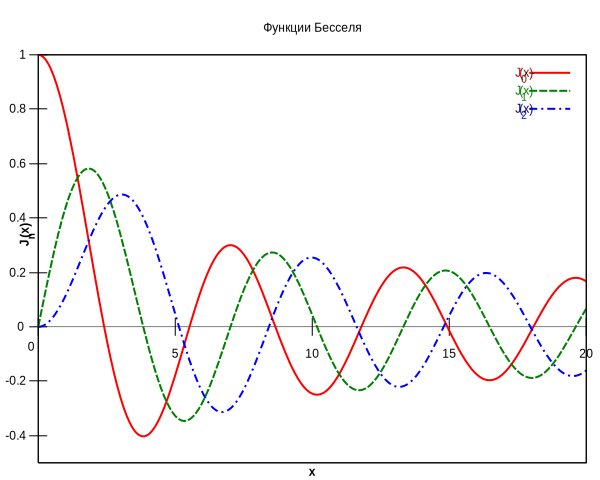
\includegraphics[width=0.8\textwidth]{img/bessel1-plot.svg}
% \end{figure}

\includesvg{bessel1-plot}

\includesvg{bessel2-plot}

По этим графикам видно\footnote{Лучше, конечно, доказать это аналитически.}, что
функция Бесселя второго рода не ограничена в нуле. Обе функции имеют счётное
количество корней --- то же касается и их производных. Функция $ J_n(x) $ при $
x\to\infty$ стремится к нулю. График функции Бесселя похож на
синусоиду, колебания которой затухают пропорционально $1/\sqrt{x}$, хотя на самом деле нули функции расположены не периодично (однако расстояние между двумя последовательными нулями стремится к 
$\pi$ при $x\to \infty $).
 \newpage
	\subsection{Собственные значения и собственные функции задачи Штурма -- Лиувилля для цилиндра. Краевые задачи для уравнений Лапласа и Пуассона в ограниченном цилиндре}
\subsubsection{Штурм -- Лиувилль}
%aut: Slava
%ref: Свешников, стр. 121 (147 2ed.)
Рассматривается задача 
\[
  \begin{cases}
    \Delta u + \lambda u = 0, & 0 < r < a, \ 0\leqslant \varphi \leqslant 2\pi,
    \ 0 < z < l,\\
    \alpha u_r(a, \varphi, z) + \beta u(a, \varphi, z) = 0,\\
    \alpha_1 u_z(r,\varphi, 0) - \beta_1 u(r,\varphi, 0) = 0,\\
    \alpha_2 u_z(r,\varphi, l) + \beta_2 u(r,\varphi, l) = 0.
  \end{cases}
\]
Напомним\footnote{См. раздел \ref{sec:14}.}, 
\[
  \Delta u(r,\varphi,z) = \Delta_2 u + u_{zz},
\]
где $ \Delta_2 $ --- оператор Лапласа на плоскости.

Разделим переменные --- $ u = v(r, \varphi) Z(z) $ --- и получим соотношение 
\[
    \frac{\Delta_2 v + \lambda v}{v} = - \frac{Z''}{Z} =: \nu.
\]
Так задача Штурма -- Лиувилля распалась на две задачи Штурма -- Лиувилля: 
\[
  \begin{cases}
    Z'' + \nu Z = 0, \quad 0 < z < l,\\
    \alpha_1Z'(0) -\beta_1 Z(0) = 0,\\
    \alpha_2 Z'(l) + \beta_2 Z(l) = 0.
  \end{cases}\quad
  \begin{cases}
    \Delta v + \varkappa = 0, \quad 0 < r < a, \ 0 \leqslant \varphi \leqslant
    2\pi,\\
    \alpha v_z(a,\varphi) + \beta v(a,\varphi) = 0,
  \end{cases}
\]
где $ \varkappa := \lambda - \nu $. Первая (одномерная) задача была решена в
разделе \ref{sec:S-L}, вторая (круговая) --- в разделе \ref{sec:20}. 

Собственные функции имеют вид 
\[
  u_{knm}(r, \varphi, z) = J_n \left( \sqrt{\varkappa_{kn}}r \right) (A_{kn}
\cos n\varphi + B_{kn} \sin n\varphi) Z_m(z),
\]
а собственные значения вычисляются по формуле $ \lambda_{knm} = \varkappa_{kn} +
\nu_m$.



\subsubsection{Лаплас}
%ref: Пикулин, стр. 32



\subsubsection{Пуассон}
%ref: Пикулин, стр. 37
 \newpage
	\subsection{Полиномы Лежандра¸их свойства. Формула Родриго. Рекуррентные соотношения. Задача Штурма – Лиувилля на сфере. Присоединенные функции Лежандра.}

%Самарский стр. 709
%aut: Денис


\textbf{Полиномы Лежандра, формула Родриго}

Полиномы Лежандра тесно связаны с ФР уравнения Лапласа $\frac{1}{R}$, где $R$ - расстояние от $М$ до $M_0$. Пусть $r, r_0$ - радиус-векторы этих точек, а $\theta$ - угол между ними

\[
\frac{1}{R}=\frac{1}{\sqrt{r_{0}^{2}+r^{2}-2 r r_{0} \cos \theta}}=\begin{cases}
	\frac{1}{r_{0}} \frac{1}{\sqrt{1+\rho^{2}-2 \rho x}} & \text { для } \quad r<r_{0}, \\
	\frac{1}{r} \frac{1}{\sqrt{1+\rho^{2}-2 \rho x}} & \text { для } \quad r>r_{0},
\end{cases}.
\]

где $x=\cos \theta(-1 \leq x \leq 1)$ и $\rho=r / r_{0}<1$ или $\rho=r_{0} / r<1$ (в обоих случаях $\rho$ меньше единицы).

Функция
\[
\Psi(\rho, x)=\frac{1}{\sqrt{1+\rho^{2}-2 \rho x}} \quad(0<\rho<1, \quad-1 \leq x \leq 1)
\]
называется производящей функцией полиномов Лежандра.

Разложим функцию $\Psi(\rho, x)$ в ряд по степеням $\rho$ :
\[
\Psi(\rho, x)=\sum_{n=0}^{\infty} P_{n}(x) \rho^{n} .
\]

Коэффициенты $P_{n}(x)$ разложения формулы являются полиномами $n$-й степени и называются полиномами Лежандра.
В силу теоремы Коши из формулы следует, что
\[
P_{n}(x)=\left.\frac{1}{n !} \frac{\partial^{n} \Psi}{\partial \rho^{n}}\right|_{\rho=0}=\frac{1}{2 \pi i} \int_{C} \frac{\Psi(\zeta, x)}{\zeta^{n+1}} d \zeta,
\]
где $C$ - любой замкнутый контур в плоскости комплексного переменного $\zeta=\xi+i \eta$, содержащей точку $\zeta=0$. Полагая $\sqrt{1-2 x \zeta+\zeta^{2}}=$ $=1-\zeta z$, находим $\zeta=2(z-x) /\left(z^{2}-1\right), d \zeta=2(1-\zeta z) d z /\left(z^{2}-1\right)$, $\Psi(\zeta, x) d \zeta=2 d z /\left(z^{2}-1\right)$.

Формула выше примет вид
\[
P_{n}(x)=\frac{1}{2^{n+1} \pi i} \int_{C_{1}} \frac{\left(z^{2}-1\right)^{n}}{(z-x)^{n+1}} d z
\]
где $C_1$ - любой контур окружающий точку $z = x$.

Учитывая, что
\[
\frac{1}{2 \pi i} \int_{C_{1}} \frac{\left(z^{2}-1\right)^{n}}{z-x} d z=\left(x^{2}-1\right)^{n},
\]

и пользуясь формулой для производной
\[
\frac{d^{n}}{d x^{n}} \int_{C_{1}} \frac{\left(z^{2}-1\right)^{n}}{z-x} d z=n ! \int_{C_{1}} \frac{\left(z^{2}-1\right)^{n}}{(z-x)^{n+1}} d z,
\]

получаем формулу для $P_{n}(x)$ :
\[
P_{n}(x)=\frac{1}{2^{n} n !} \frac{d^{n}}{d x^{n}}\left[\left(x^{2}-1\right)^{n}\right] .
\]

Формула называется дифференциальной формулой для полиномов Лежандра или формулой Родрига.

Из данной формулы непосредственно видно, что: 1) $P_{n}(x)$ есть полином степени $n ; 2) P_{n}(x)$ содержит только степени $x$ той четности, что и номер $n$, так что
\[
P_{n}(-x)=(-1)^{n} P_{n}(x) .
\]

Полагая $x=1$, находим
\[
\Psi(\rho, 1)=\frac{1}{1-\rho}=1+\rho+\ldots+\rho^{n}+\ldots=\sum_{n=0}^{\infty} P_{n}(1) \rho^{n},
\]
т. е. $P_{n}(1)=1$, и в силу $(7)$
\[
P_{n}(-1)=(-1)^{n} .
\]


\textbf{Рекуррентные формулы. }

Дифференцируя $\Psi(\rho, x)$ по $\rho$ и $x$, получаем два тождества:
\[
\begin{aligned}
	\left(1-2 \rho x+\rho^{2}\right) \Psi_{\rho}-(x-\rho) \Psi=0, \\
	\left(1-2 \rho x+\rho^{2}\right) \Psi_{x}-\rho \Psi=0 .
\end{aligned}
\]

Запишем в виде степенного ряда относительно $\rho$, подставив в нее ряд $\Psi(\rho, x)=\sum_{n=0}^{\infty} P_{n}(x) \rho^{n}$ для $\Psi$ и ряд $\Psi_{\rho}=\sum_{n=0}^{\infty}(n+1) P_{n+1}(x) \rho^{n}$.
Коэффициент при $\rho^{n}$ полученного ряда равен нулю при всех $x$ :
\[
(n+1) P_{n+1}(x)-x(2 n+1) P_{n}(x)+n P_{n-1}(x)=0 .
\]

Это тождество есть рекуррентная формула, связывающая три последовательных полинома. Она позволяет найти последовательно все $P_{n}(x)$ $(n>1)$, если учесть, что
\[
P_{0}(x)=1, \quad P_{1}(x)=x .
\]

Так, например, полагая $n=1$, находим $P_{2}(x)=1 / 2 \cdot\left(3 x^{2}-1\right)$.
Выведем еще две рекуррентные формулы:
\[
n P_{n}(x)-x P_{n}^{\prime}(x)+P_{n-1}^{\prime}(x)=0,
\]

или
\[
\begin{array}{c}
	P_{n-1}^{\prime}(x)=x P_{n}^{\prime}(x)-n P_{n}(x), \\
	P_{n}^{\prime}(x)-x P_{n-1}^{\prime}(x)-n P_{n-1}(x)=0 .
\end{array}
\]

\textbf{Присоединенные функции Лежандра}

Рассмотрим следующую задачу. Найти собственные значения и собственные функции уравнения
\[
\frac{d}{d x}\left[\left(1-x^{2}\right) \frac{d y}{d x}\right]+\left(\lambda-\frac{m^{2}}{1-x^{2}}\right) y=0, \quad-1<x<1,
\]

при условии ограниченности
\[
|y( \pm 1)|<\infty .
\]

Решение уравнение естественно искать в виде
\[
y(x)=\left(1-x^{2}\right)^{m / 2} v(x), \quad v( \pm 1) \neq 0 .
\]

Подставив в исходное, найдем
\[
\left(1-x^{2}\right) v^{\prime \prime}-2(m+1) v^{\prime}+[\lambda-m(m+1)] v=0 .
\]

Нетривиальное ограниченное решение $z=P_{n}(x)$ уравнения Лежандра существует лишь при $\lambda=n(n+1)$, где $n$ - целое положительное число. Отсюда следует, что
\[
v(x)=\frac{d^{m} P_{n}}{d x^{m}}, \quad \lambda=n(n+1)
\]

есть решение уравнения, а функция
\[
P_{n}^{(m)}(x)=\left(1-x^{2}\right)^{m / 2} \frac{d^{m} P_{n}}{d x^{m}}
\]
есть собственная функция задачи, соответствующая собственному значению
\[
\lambda_{n}=n(n+1), \quad n=1,2, \ldots
\]

Функция $P_{n}^{(m)}(x)$ называется присоединенной функцией Лежандра $m$ го порядка.

Согласно общей теореме присоединенные функции $P^{(m)}_n$ образуют ортогональную систему. Тогда квадрат нормы присоединенних функций равен:

\[
||P^{(m)}_n||^2 = \frac{2}{2n+1}\frac{(n+m)!}{(n-m)!}
\]

 \newpage
	\subsection{Краевые задачи для уравнений Лапласа и Пуассона в шаровом слое.}

Вот такое уравнение называется первой краевой задачей для уравнения Пуассона в шаровом слое:
\[
  \begin{cases}
    \Delta u = f(x, y, z), (x, y, z) \in \Omega, \\
    \left. u \right|_{r = a} = g(\varphi, \theta), \\
    \left. u \right|_{r = b} = h(\varphi, \theta),
  \end{cases}
\]
где $\Omega = \left\{ (r, \theta, \varphi) : a < r < b \right\} $.
При $f(x, y, z) \equiv 0$ уравнение называется Лапласом.

Если на границах заданы производные вдоль внешней нормали, то это вторая краевая задача,
а если задана линейная комбинация, то это третья краевая задача.

\paragraph{Способы решения}
\begin{itemize}
  \item Найти частное решение $w$ для неоднородного уравнения, то есть найти какое-нибудь 
    решение задачи $\Delta w = f(x, y, z)$. Чаще всего такое можно сделать, если правая часть 
    представляется в каком-то специальном виде, например,
    если $f(x, y, z) = r^2 \cos 2\varphi$, то $w$ легко ищется в виде $A r^\alpha \cos 2\varphi$,
    если $f(x, y, z) = \operatorname{const}$, то $w = A r^\alpha$.
    Тогда останется найти только часть решения $v$, удовлетворяющую уравнению:
    \[
      \begin{cases}
        \Delta v = 0, \\
        \left. v \right|_{r=a} = g(\varphi, \theta) - \left. w \right|_{r=a}, \\
        \left. v \right|_{r=b} = h(\varphi, \theta) - \left. w \right|_{r=b}.
      \end{cases}
    \]

  \item Метод функций Грина.
    % TODO про функции Грина не разбираюсь

  \item Метод разделения переменных, о нём ниже.
\end{itemize}

\paragraph{Разделение переменных}

Если представить решение в виде: $u = R(r) W(\varhpi, \theta)$, то
\begin{multline*}
  \left( r^2 R' \right)' W
  + \dfrac{1}{\sin \theta} R \dfrac{\partial }{\partial \theta} \left( \sin\theta \dfrac{\partial W}{\partial \theta} \right) 
  + \dfrac{1}{\sin^2 \theta} R \dfrac{\partial^2 W}{\partial \varphi^2} = 0
  \Rightarrow \\
  \Rightarrow
  \dfrac{(r^2 R')'}{R}
  = - \dfrac
    {\dfrac{1}{\sin \theta} \dfrac{\partial }{\partial \theta} \left( \sin\theta \dfrac{\partial W}{\partial \theta} \right) + \dfrac{1}{\sin^2 \theta} \dfrac{\partial^2 W}{\partial \varphi^2}}
    {W} = - \lambda
\end{multline*}
далее разделим $W = \Theta(\theta) \Phi(\varphi)$:
\[
  \sin\theta \Phi (\sin\theta \Theta')' + \lambda \sin^2\theta \Theta\Phi
  + \Theta \Phi'' = 0
  \Rightarrow
  - \dfrac{\sin\theta (\sin\theta \Theta')' + \lambda \sin^2\theta \Theta}{\Theta}
  = \dfrac{\Phi''}{\Phi} = -\mu,
\]
решением задачи для $\Phi(\varphi)$ с дополнительным условием однозначности является:
\[
  \Phi_n (\varphi) = a_n \cos(n \varphi) + b_n \sin(n \varphi), \mu = n^2,
  n \in \mathbb{N} \cup \{0\}
\]
Тогда задача для $\Theta$ принимает вид:
\[
  \begin{cases}  
    \sin\theta (\sin\theta \Theta')' + \lambda \sin^2\theta \Theta - n^2 \Theta = 0, \\
    |\Theta(0)| < \infty, |\Theta (\pi)| < \infty.
  \end{cases}
\]
Решением такой задачи являются полиномы Лежандра (это надо проверить):
\[
  \Theta_{nm} (\theta) = P_{m}^{(n)} (\cos\theta),
  \lambda_m = m(m+1), m \in \left\{ 0, 1, \dots, n \right\} 
\]

Теперь можно вернуться к неоднородной задаче, так как мы получили ортогональную систему.
 \newpage
	\subsection{Основные функции и обобщенные функции, сходимость в пространстве основных функций. Регулярная обобщённая функция. Носитель обобщённой функции}
%aut: Slava
%ref: Владимиров, стр. 65
\subsubsection{Основа}
\textsc{Пример мотивации.} Найти плотность материальной точки. Интеграл
плотности по
области, содержащей эту точку должен давать её массу.

Рассмотрим однородный шар $ U_\delta $ в пространстве\footnote{Для удобства
вектор $ \mathbf x $ будет записываться как просто $ x $.} $ \mathbb R^3 $ массы $ m = 1 $ в начале координат. Плотность этого шара выражается
соотношениями\footnote{См. формулу объёма шара.}  
\[
  f_\delta(x) = \begin{cases}
    0, & |x| > \delta,\\
    \dfrac{3}{4\pi \delta^3}, & |x| < \delta.
  \end{cases}
\]
Теперь нужно устремить его радиус $ \delta \to 0 $. Классический предел не
даёт вменяемого результата, поэтому рассмотрим \emph{слабый предел}. Именно, для
каждой непрерывной функции $ \varphi $ найдём предел 
\[
  \lim_{\delta \to 0} \int f_\delta(x)\varphi(x) \, dx = \varphi(0).
\]
Действительно, для любого $ \varepsilon > 0 $ имеем такую $ \delta_0 $, что при
всех $ \delta < \delta_0 $ 
\begin{multline*}
    \left| \int f_\delta(x)\varphi(x)\, dx - \varphi(0) \right| =
    \frac{3}{4\pi\delta^3} \left| \int_{|x| < \delta} \varphi(x) - \varphi(0)\,dx
    \right| \leqslant\\\leqslant
    \frac{3}{4\pi\delta^3} \int_{|x|<\delta}|\varphi(x)-\varphi(0)|\, dx <
    \varepsilon \frac{3}{4\pi\delta^3} \int_{|x| <\delta} dx = \varepsilon.
\end{multline*}
Здесь была использована непрерывность $ \varphi $, а также общие свойства
интегралов.

\sloppy
Назовём тогда \emph{$ \delta $-функцией Дирака} полученный
функционал\footnote{<<Настоящий>> аргумент $ \delta $ --- функция. Запись $
\delta(x) $ удобна и обоснована. Применение функционала к функции будем записывать как ($\delta,
\varphi  $).} $ \delta(x)\colon C(\mathbb R^3) \to \mathbb R $, $(\delta, \varphi) = \lim\int
f_\delta\varphi\,dx = \varphi(0)$. Для точки массой $ m $ находящейся в
$ x_0  $ имеем плотность $
m\delta(x - x_0) $. Чтобы получить её массу, подействуем нашей функцией $ (m\delta, 1)
= m\cdot1(x_0) = m$ на $ \varphi\equiv 1 $. Полученный функционал линеен и
непрерывен в смысле нормы $ L_2 $. Функционалы с такими свойствами и называют
\emph{обобщёнными функциями}.

\subsubsection{Пространство основных функций $ \mathcal D $} Функция $ \varphi $ в
нашем примере, как говорят, является \emph{основной функцией} для $ \delta(x) $.
Она достаточно хороша, чтобы соответствующий предел существовал. Ясно, что чем
<<лучше>> пространство основных функций, тем больше существует линейных непрерывных
функционалов на нем. 

Пространство основных функций $ \mathcal D = \mathcal D(\mathbb R^n) $ ---
все финитные\footnote{Носитель --- замыкание множества, на котором функция
отлична от нуля (обозн. $ \operatorname{supp} $) --- компактен (ограничен).} бесконечно дифференцируемые в $
\mathbb R^n $ функции вместе с введённым понятием сходимости.

\paragraph{Сходимость в $ \mathcal D $.} Скажем, что последовательность функций $ \varphi_k \in
\mathcal D$ сходится к функции $ \varphi \in \mathcal D $, если 
\begin{enumerate}
  \item Существует такое число $ R > 0 $, что $ \operatorname{supp} \varphi_k \subset U_R $.
  \item Для любого мультииндекса $ \alpha = (\alpha_1, \alpha_2, \ldots,
    \alpha_n) $ выполняется\footnote{Обозначения: $\alpha_k = 0, 1, \ldots$;
    $|\alpha| := \sum \alpha_k$; $\partial^\alpha f(x) :=
  \frac{\partial^{|\alpha|}f(x_1, \ldots, x_n)}{\partial x_1^{\alpha_1}
\ldots\partial_n^{\alpha_n}}$. Знаком $ \rightrightarrows $ обозначается
равномерная сходимость: $ \exists \delta \forall\varepsilon\colon |x-x_0| < \delta
\Rightarrow |f(x) - f(x_0)| < \varepsilon $.} 
  \[
      \partial^\alpha \varphi_k(x) \rightrightarrows \partial^\alpha\varphi(x),
      \quad k \to \infty.
  \]
\end{enumerate}

\paragraph{Примеры непрерывных операторов на $ \mathcal D $.} 
\begin{enumerate}
  \item Докажем по определению\footnote{Определение: $ f_k \to f
      \Rightarrow Lf_k \to Lf $, что равносильно ($ g_k = |f - f_k| $) $ g_k \to 0
    \Rightarrow Lg_k \to 0 $.} непрерывность оператора дифференцирования, то есть
    что $ \varphi_k \to 0 $ влечёт $
    \partial^\alpha\varphi_k \to 0 $. Первое требование выполняется очевидным
    образом. Второе требование следует из соотношения $ \partial^\beta \circ
    \partial^\alpha = \partial^{\alpha + \beta} $.
  \item Аналогично показывается, что непрерывен оператор $ (l, \varphi(x)) :=
    \varphi(Ax + B) $, $ A \neq 0 $.
  \item  Непрерывна операция умножения на функцию\footnote{$C^\infty(\mathbb
      R^n)$ есть
    пространство бесконечно дифференцируемых на $ \mathbb R^n $ функций.} $
  a(x)\in C^\infty(\mathbb R^n) $.
\end{enumerate}
Заметим, что все перечисленные операции переводят функции из $ \mathcal D $ в
функции из $ \mathcal D $ (это обособленные факты).
 \newpage
	\subsection{Регуляризация степенных особенностей. Сингулярная обобщённая функция $\mathcal{P} \frac{1}{x}$. Формула Сохоцкого.} \newpage
	\subsection{Фундаментальное решение дифференциального оператора. Обобщённое решение задачи Коши.}

Написанное ниже взято из Владимирова, страницы 144--147.

Обозначения:
\begin{itemize}
  \item $\mathcal{D}$ -- пространство (обычных) основных функций: финитные бесконечно
    дифференцируемые в $\mathbb{R}^n$ функции; 
  \item $\mathcal{D}'$ -- пространство (обычных) обобщённых функций;
  \item $\mathcal{S}$ -- пространство основных функций медленного роста: все бесконечно
    дифференцируемые функции на $\mathbb{R}^n$, убывающие при $|x| \to \infty$ вместе со
    всеми производными быстрее любой степени $|x|^{-1}$;
  \item $\mathcal{S}'$ -- пространство обобщённых функций медленного роста;
\end{itemize}

\paragraph{Фундаментальное решение}
ОПРЕДЕЛЕНИЕ. Пусть $L$ -- дифференциальный оператор с постоянными коэффициентами,
$a_\alpha (x) = a_\alpha = \operatorname{const}$,
\[
  L(\partial) = \sum_{|\alpha| = 0}^m a_\alpha \partial^\alpha, L^* (\partial) = L(-\partial).
\]
\emph{Фундаментальным решением (функцией влияния)} оператора $L(\partial)$ называется обобщенная
функция $\mathcal{E} \in \mathcal{D}' (\mathbb{R}^n)$, удовлетворяющая в $\mathbb{R}^n$ 
уравнению
\[
  L(\partial) \mathcal{E} = \delta (x).
\]

Оно не единственно и определяется с точностью до слагаемого
$\mathcal{E}_0: L(\partial) \mathcal{E}_0 = 0$.

Верна следующая лемма:
\begin{theorem}
  \[
    \mathcal{E} \in \mathcal{S}' \text{-- фундаментальное решение $L(\partial)$}
    \Leftrightarrow
    L(-i \xi) F[\mathcal{E}] = 1,
  \]
  где $L(\xi) = \sum_{|\alpha|=0}^m a_\alpha \xi^\alpha$, $F[\mathcal{E}]$ -- преобразование Фурье.
\end{theorem}

Эта лемма следует из свойств преобразования Фурье. Из этой леммы мы знаем о том, каким образом можно
находить фундаментальные решения, а так же знаем, что они не единственны в силу не единственности 
решений получаемых алгебраических уравнений. Так же было доказано, что получаемое уравнение всегда разрешимо в классе $\mathcal{S}'$, если $L(-i\xi)$ не равно тождественно нулю.


\begin{theorem}[Теорема о решении уравнения с правой частью]
  Пусть $f \in \mathcal{D}'$ такова, что $\exists \mathcal{E} * f \in \mathcal{D}'$. Тогда решение
  уравнения $L(\partial) u = f(x)$ существует в $\mathcal{D}'$ и даётся формулой
  \[
    u = \mathcal{E} * f.
  \]
  Причём это решение единственно в классе тех обобщённых функций из $\mathcal{D}'$, для которых
  существует свёртка с $\mathcal{E}$.
\end{theorem}
Эта теорема следует из свойств дифференцирования свёртки.



\paragraph{Обобщённое решение задачи Коши} \footnote{(Владимиров, стр 168)}
Сформулируем задачу Коши: оператор $L = \sum_{k=0}^m a_k \dfrac{d}{dx^k}$:
\[
  \begin{cases}
    Ly = f(x), x > 0, f \in \mathcal{C} \\
    y(0) = a_0, \\
    y'(0) = a_1, \\
    \dots \\
    y^{(m-1)} (0) = a_{(m-1)}.
  \end{cases}
\]
% TODO недописано



Обозначим за $Z(x)$ решение однородного уравнения:
\[
  \begin{cases}
    LZ = 0, \\
    Z(0) = Z'(0) = \dots = Z^{(m-2)} (0) = 0, \\
    Z^{(m-1)} (0) = 1.
  \end{cases}
\]
(на всякий случай, такое решение будет в виде: $Z(x) = \sum e^{\lambda_k x}$)

Покажем, что 


Так же вот табличка основных фундаментальных решений:
\begin{center}
  \begin{tabular}{|c|c|}
    \hline
    Оператор & фундаментальное решение \\
    \hline
    теплопроводности $\dfrac{\partial \mathcal{E}}{\partial t} - a^2 \Delta \mathcal{E}$ &
    $\mathcal{E} (x, t) = \dfrac{\theta(t)}{(2a \sqrt{\pi t})^n} \exp \left\{ -\dfrac{|x|^2}{4a^2 t} \right\}$ \\
    
    \hline
    Лаплас $\Delta \mathcal{E}$ &
    $\mathcal{E}_2 = \dfrac{1}{2\pi} \ln |x|, \mathcal{E} = -\dfrac{1}{(n-2) \sigma_n} |x|^{-n+2}$ \\
    \hline 
    Гельмгольца $(\Delta + k^2) \mathcal{E}_n$ &
    $\mathcal{E}_1 (x) = \dfrac{1}{2ik} e^{ik |x|}, \bar\mathcal{E}_1 (x) = - \dfrac{1}{2ik} e^{-ik|x|}$ \\
    \hline
  \end{tabular}
\end{center}


 \newpage
	\subsection{Классическая свёртка. Свертка обобщённых функций. Обобщённое решение дифференциального уравнения.} \newpage
	\subsection{Пространство быстроубывающих функций и пространство функций медленного роста.
Обобщённое преобразование Фурье. Обобщённое преобразование Фурье свертки и обобщённое равенство
Парсеваля.}
\label{question:30}

\subsubsection{Пространство функций медленного роста}

ОПРЕДЕЛЕНИЕ. Пространство основных функций $\mathcal{S}$ определим следующим образом: это все
функции класса $\mathcal{C}^\infty (\mathbb{R}^n)$, убывающие при $|x| \to \infty$ вместе со всеми
производными быстрее $|x|^{-k}$. Сходимость в $\mathcal{S}$ определим следующим образом:
последовательность функций $\varphi_k \in \mathcal{S}$ сходится к функции
$\varphi \in \mathcal{S}, \varphi_k \to \varphi, k \to \infty \text{ в } \mathcal{S}$, если для
всех $\alpha, \beta$
\[
  x^\beta \partial^\alpha \varphi_k (x) \rightrightarrows x^\beta \partial^\alpha \varphi(x), x\in\mathbb{R}^n, k \to \infty.
\]

Это пространство получается замкнутым относительно дифференцирования:
$\forall \varphi \in \mathcal{S} \forall \alpha : \partial^\alpha \varphi \in \mathcal{S}$.
Но что было хорошо с пространством $\mathcal{D}$, так это то, что оно было замкнуто относительно
умножения на любую бесконечно-дифференцируемую функцию:
$\forall \varphi \in \mathcal{D} \forall f \in \mathcal{C}^\infty (\mathbb{R}^n) : \varphi(x) \cdot f(x) \in \mathcal{D}$. Такого нельзя сказать про пространство $\mathcal{S}$, однако если чуть
сузить класс функций, на которые мы хотим уметь умножать, то получим пространство функций медленного
роста (????):
\[
  \Omega_M = \left\{ a\in\mathcal{C}^\infty(\mathbb{R}^n) :
    \forall\alpha : \left| \partial^\alpha a(x) \right|
      \leqslant C_\alpha (1+|x|)^{m(\alpha)} \right\} 
\]

ОПРЕДЕЛЕНИЕ. Пространством обобщённых функций медленного роста называется пространство линейных
непрерывных функционалов над $\mathcal{S}$.

Верна следующая теорема:
\begin{theorem}[Л. Шварц]
  Для того, чтобы линейный функционал $f$ на $\mathcal{S}$ принадлежал $\mathcal{S}'$ (т.е. был
  непрерывным на $\mathcal{S}$), необходимо и достаточно, чтобы существовали число $C>0$ и целое
  число $p\geqslant 0$ такие, что
  \[
    |(f, \varphi)| \leqslant C \|\varphi\|_p
  \]
  для любой $\varphi \in \mathcal{S}$, где
  \[
    \|\varphi\|_p = \sup_{|\alpha| \leqslant p, x\in\mathbb{R}^n} (1+|x|)^p |\partial^\alpha \varphi(x)|.
  \]
\end{theorem}

Пользуясь теоремой Л. Шварца, можно доказать, что всякая обобщенная функция из $\mathcal{S}'$
является производной (в смысле обобщённых функций) от непрерывной функции медленного роста. Этим и
объясняется название пространства $\mathcal{S}'$.

\paragraph{Плотность $\mathcal{D}$ в $\mathcal{S}$}\footnote{Владимиров Жаринов, стр. 119}

Плотность $A$ в $B$ означает, что для любой $b \in B$ найдётся последовательность $a_n \in A$ такая,
что $a_n \to b, n \to \infty$ в $B$.

Для доказательства утверждения плотности $\mathcal{D}$ в $\mathcal{S}$, выберем какую-то функцию
$\varphi \in \mathcal{S}$, тогда последовательность
$\varphi_k(x) = \varphi(x) \eta(\dfrac{x}{k}) \in \mathcal{D}$, где $\eta \in \mathcal{D}$ и
$\eta(x) = 1, |x| < 1$, сходится к $\varphi$ в $\mathcal{S}$.

\subsubsection{Преобразование Фурье}

Это интегральное преобразование, которое действует по формуле:
\[
  F[f(\vec{x})](\vec{\xi}) = \int_{\mathbb{R}^n} f(\vec{\xi}) e^{i (\vec{x},\vec{\xi})} \, d\vec{\xi}
\]
Также можно взять преобразование только по какой-то части координат, это обозначается так:
$x = (i_1, i_2, \dots, i_k), k < n$:
\[
  F_x [f(\vec{x})] (\xi) = \int_{\mathbb{R}^k} f(\vec{\xi}) e^{i (\vec{x}, \vec{\xi})} \, d\vec{\xi}
\]

\subsubsection{Преобразование Фурье обобщённых функций из $\mathcal{S}'$}

Определим преобразование Фурье обобщённой функции так, чтобы выполнялось соотношение
\[
  (F[f], \varphi) = (f, F[\varphi]), \varphi \in \mathcal{S}.
\]
делаем именно так, чтобы если подставить вместо $f$ что-то обычное, получалось бы верное равенство:
\begin{multline*}
  \int F[f] \varphi \, d\xi
  = \int \left( \int f(x) e^{i (\xi, x)} \, dx \right) \varphi(\xi) \, d\xi
  = \int f(x) \left( \int \varphi(\xi) e^{i (x, \xi)} \, d\xi \right) \, dx
  = \int f(x) F[\varphi](x) \, dx.
\end{multline*}

Введём на $\mathcal{S}'$ еще операцию $F^{-1}$:
\[
  F^{-1}[f] = \dfrac{1}{(2\pi)^n} F[f(-x)], f\in\mathcal{S}'.
\]

Из важного:
\begin{itemize}
  \item 
    \[
      \partial^\alpha F[f] = F \left[ (ix)^\alpha f(x) \right].
    \]
  \item
    \[
      F \left[ \partial^\alpha f \right] (\xi) = (-i\xi)^\alpha F[f] (\xi).
    \]
  \item Преобразование Фурье свёртки
    \[
      F \left[ f * g \right] = F[f] \cdot F[g]
    \]
\end{itemize}

\subsubsection{Равенство Парсеваля}

Вот такое соотношение обычно называют равенством Парсеваля \footnote{Гельфанд, Шилов -- Обобщённые функции и действия над ними, стр. 210}:
\begin{multline*}
  (f, \varphi) = \int f \varphi \, dx = \int f(x) F^{-1} [ F[\varphi] ] (x) \, dx
  = \int_{\mathbb{R}^n} f(x) \dfrac{1}{2\pi}\int_{\mathbb{R}^n} F[\varphi] (\xi) e^{-ix \xi} \, d\xi dx = \\
  = \dfrac{1}{2\pi}\int_{\mathbb{R}^n} F[\varphi](\xi) \int_{\mathbb{R}^n} f(x) e^{-ix \xi} \, dx d\xi
  = \int_{\mathbb{R}^n} F[\varphi](\xi) F^{-1} [f] (\xi) \, d\xi
  = (F^{-1} [f], F[\varphi])
\end{multline*}
 \newpage
	\subsection{Фундаментальное решение оператора Лапласа.} \newpage
	\subsection{Фундаментальное решение оператора теплопроводности. Функция влияния мгновенного точечного источника.} \newpage
	\subsection{Фундаментальное решение оператора Гельмгольца. Сферические волны.} \newpage
	
	\section{Дополнение}
	
	\subsection{Штурм-Лиувилль. Дополнительные сведения.}

Имеем задачу на собственные значения 
\begin{align}
	\Delta u + \lambda \rho u = 0, \label{shturm} \\
	u|_{S} = 0 \label{liouville}
\end{align}

Утверждается, что:
\begin{enumerate}
	\item Существует бесконечное счетное множество собственных значений
	\begin{equation}
		\lambda_1 \leqslant \lambda_2 \leqslant \dotsc \leqslant \lambda_n \leqslant \dotsc
	\end{equation}
	
	\item Все собственные значения положительны $\lambda_n > 0$. Обозначим через $\{u_n(M)\}$ множество собственных значений функций задачи \eqref{shturm}--\eqref{liouville}:
	\begin{equation*}
		v_n(M) = \sqrt{\rho(M)} u_n(M).
	\end{equation*}
	
	Воспользуемся первой формулой Грина:
	\begin{equation*}
		\int \limits_{D} u_n \Delta u_n \, dV = \oint \limits_{S} u_n \frac{\partial u_n}{\partial n} \, dS - \int \limits_{D} (\nabla u_n)^2 \, dV.
	\end{equation*}
	Поскольку $\Delta u_n = - \lambda_n \rho u_n, u_n|_{S} = 0$, то 
	\begin{equation} \label{eqforsl}
		\lambda_n \int \limits_{D} \rho u_n^2 \, dV = \int \limits_{D} (\nabla u_n)^2 \, dV.
	\end{equation}
	Отсюда сразу следует, что $\lambda_n > 0$ при всех $n$. 
	
	Заметим, что для задачи Штурма-Лиувилля с граничным условием Неймана из \eqref{eqforsl} следует, что она имеет наименьшее нулевое собственное значение. С этим обстоятельством связана неединственность решения внутренней задачи Неймана для уравнения Лапласа. Наконец, заметим, что в случае Штурма-Лиувилля с третьим граничным условием ($\frac{\partial u}{\partial n} + h u |_{s} = 0$) при отрицательной функции $h(P) < 0$ задача может иметь конечное число отрицательных значений $\lambda_n$. 
	
	\item Собственные функции ортогональны в области $D$ с весом $\rho(M)$:
	\begin{equation}
		\int \limits_{D} u_n u_m \rho \, dV = 0 \text{ при } n \not = m.
	\end{equation}
\end{enumerate}

\begin{theorem}[В.А. Стеклов]
	Всякая функция $f$ разлагается в регулярно сходящийся ряд Фурье по собственным функциям $\{X_k\}$ задачи Штурма-Лиувилля:
	\begin{equation*}
		f(x) = \sum \limits_{k = 1}^{\infty} (f, X_k) X_k(x).
	\end{equation*}
\end{theorem}
 \newpage
	
\end{document}
